%% Elsevier / Reliability Engineering & System Safety (RESS) submission.
%% Template source: official Elsevier elsarticle package (CTAN, Copyright 2007-2026).
\documentclass[preprint,12pt]{elsarticle}

\usepackage{amssymb}
\usepackage{amsmath}
\usepackage{booktabs}
\usepackage{array}
\usepackage{longtable}
\usepackage{tabularx}
\usepackage{xltabular}
\usepackage{makecell}
\usepackage{enumitem}
\usepackage[protrusion=true,expansion=false]{microtype}
\usepackage{xurl}
\usepackage{float}

\newcolumntype{Y}{>{\raggedright\arraybackslash}X}
\sloppy
\setlength{\emergencystretch}{3em}

%% Float placement: keep full-width tables near their first mention instead of
%% deferring tall floats to the end of the document.
\renewcommand{\topfraction}{0.9}
\renewcommand{\bottomfraction}{0.8}
\renewcommand{\textfraction}{0.07}
\renewcommand{\floatpagefraction}{0.7}
\setcounter{topnumber}{3}
\setcounter{totalnumber}{5}

\journal{Reliability Engineering \& System Safety}

\begin{document}

\begin{frontmatter}

\title{Domain-Validity-Gated Verification of Machine-Learning Surrogates: Auditable Fault Attribution for Out-of-Distribution Use}

\author[inst1,inst2,inst3]{Meng Li\corref{cor1}\fnref{orcid-ml}}
\ead{mlemon@usc.edu.cn}
\author[inst1,inst2,inst3]{Xiaohua Yang\fnref{orcid-xy}}
\ead{xiaohua1963@foxmail.com}
\author[inst1,inst2,inst3]{Jie Liu\fnref{orcid-jl}}
\ead{jieliu@usc.edu.cn}
\author[inst1,inst2,inst3]{Shiyu Yan\fnref{orcid-sy}}
\ead{yanshiyu@usc.edu.cn}
\cortext[cor1]{Corresponding author: Meng Li.}
\fntext[orcid-ml]{ORCID: Meng Li, 0000-0002-1074-1502.}
\fntext[orcid-xy]{ORCID: Xiaohua Yang, 0000-0002-2977-1787.}
\fntext[orcid-jl]{ORCID: Jie Liu, 0009-0008-1970-8347.}
\fntext[orcid-sy]{ORCID: Shiyu Yan, 0000-0001-7626-5185.}
\affiliation[inst1]{organization={School of Computing, University of South China},
  city={Hengyang}, postcode={421001}, country={China}}
\affiliation[inst2]{organization={Hunan Engineering Research Center of Software Evaluation and Testing for Intellectual Equipment},
  city={Hengyang}, postcode={421001}, country={China}}
\affiliation[inst3]{organization={CNNC Key Laboratory on High Trusted Computing},
  city={Hengyang}, postcode={421001}, country={China}}

\begin{abstract}
Machine-learning surrogates are increasingly deployed as components of complex engineering systems, where they must be trusted on operating points far from their training distribution. Unlike the high-fidelity models they replace, such surrogates have no cheap exact oracle, so a failed check cannot easily be attributed to a genuine surrogate fault rather than an inapplicable test or a numerical artifact, a recurring obstacle for verification, fault detection, and diagnosis. We present a domain-validity-gated method that turns physically derived consistency relations into auditable, executable verification assets and decides, before any fault is reported, whether a relation is admissible for a given surrogate: its preconditions must hold, its measuring operator must be numerically decidable so that the tolerance dominates the operator's intrinsic error floor, and its verdict is typed to separate a true surrogate inconsistency from out-of-domain application and numerical limits. A claim ledger binds every reported result to a recorded artifact. On a mesh-based computational-fluid-dynamics surrogate, with supporting cross-architecture and cross-equation studies, the gate removes detectors that would false-alarm on a correct surrogate, rejects physically inapplicable relations, and bounds where the admitted checks can and cannot surface seeded faults. The outcome is a more auditable, false-alarm-controlled basis for attributing surrogate faults.
\end{abstract}

\begin{highlights}
\item Validity gate decides when a physics check can soundly fault a learned surrogate
\item Tolerance must dominate the measuring operator's numerical floor to admit a check
\item Typed verdicts separate surrogate faults from out-of-domain and numerical limits
\item A claim ledger binds every reported verdict to a recorded artifact
\item Case study bounds where admitted checks can and cannot surface seeded faults
\end{highlights}

\begin{keyword}
Machine-learning surrogates \sep metamorphic relations \sep oracle-free verification \sep fault attribution \sep out-of-distribution validation \sep numerical decidability \sep MeshGraphNets
\end{keyword}

\end{frontmatter}

\section{Introduction}
\label{sec:introduction}

Scientific machine-learning (SciML) surrogates are increasingly embedded as components of complex engineering systems: trained on simulator or sensor data, they replace expensive physical or numerical models inside design, monitoring, and decision pipelines \citep{raissi2019pinn,karniadakis2021piml,li2021fno}. Mesh-based neural simulators such as MeshGraphNets (MGN), which predict physical fields on irregular meshes \citep{pfaff2021meshgraphnets}, are a representative such surrogate. Once embedded, a surrogate must be trusted at operating points far from its training distribution, where its errors are least understood and where an unnoticed fault propagates into whatever system consumes its output. Unlike the high-fidelity model it replaces, a learned surrogate has no cheap exact oracle: for most inputs there is no reference answer to check against, the test oracle problem \citep{barr2015oracle}, so held-out rollout accuracy alone cannot tell an engineer whether the surrogate has violated a relation that the underlying physics requires.

A practical response is to check \emph{relations} that any correct surrogate must satisfy under controlled transformations, such as conservation, symmetry, nondimensional similarity, and continuity, instead of checking each output against a known value. This is metamorphic testing (MT), which addresses the oracle problem by relating multiple executions rather than predicting one expected output \citep{chen1998metamorphic,segura2016survey}; such physics-derived candidate metamorphic relations (MRs) are widely available for scientific software \citep{kanewala2019scientific,lin2020exploratory,olsen2019simulation} and give an oracle-free signal for fault detection when one fails. The testing problem considered in this paper begins after such candidates have been proposed. A physics-derived relation is not automatically a sound software test: mirror symmetry may depend on geometry and boundary labels; a divergence relation may depend on a discrete operator, mesh weights, and boundary treatment; a transformed case may leave the relation's validity domain before it reveals any genuine fault. Treating every failed check as a surrogate fault therefore risks false alarms and misattribution, blaming the model when the test, not the model, was at fault. The problem this paper addresses is how to decide, \emph{before} a fault is reported, whether a physically derived relation is an admissible, numerically decidable check for a given surrogate, so that its verdict can be trusted to separate a true surrogate inconsistency from an inapplicable relation or a numerical artifact.

For SciML surrogate software, this creates an interpretability problem for oracle-free verification-and-validation (V\&V): when an MR check fails, the tester must ask whether the system under test (SUT) violated a genuine relation, the relation was applied outside its validity conditions, the output mapping was incompatible with the software representation, or the scoring operator could not resolve the claimed effect. Treating all such outcomes as ordinary pass/fail MT verdicts makes the evidence hard to audit and easy to overclaim.

This paper therefore reframes SciML MR use as \emph{validity-gated V\&V asset construction}, and its thesis is that admissibility gating \emph{changes} V\&V outcomes rather than merely annotating them: the gate removes detectors that would raise false alarms on a correct surrogate, and rejects on physical grounds a relation it would only defer under different physics, so a downgraded or rejected relation is reported as out-of-distribution stress evidence rather than licensed as a SUT fault verdict. It does not claim to invent MT, and it does not replace residual, uncertainty, accuracy, or trust-region diagnostics; its contribution is to turn physics-derived candidate relations into auditable assets by combining measurement-floor admissibility, structured MR executable records, and typed verdict ledgers. Physical knowledge, expert reasoning, large language model (LLM)-assisted candidate lists, and prior physics-derived relation catalogs \citep{li2026noether} may all suggest candidate relations. The method is a verification and fault-attribution technique with a discernible relationship to the reliability of complex systems that embed learned surrogates; the evidence supports bounded SciML V\&V utility rather than general SciML reliability or real-world defect-detection rates.

Two principles organize the method. First, an MR is \emph{admissible} only when its validity conditions hold for the SUT and the verdict is numerically decidable: the tolerance must dominate the intrinsic floor of the measuring operator (machine precision, a mapping floor, or a discretization floor, by relation type). Second, relation-level verdicts are interpreted along two axes, relation-violation and domain-violation magnitude, separating SUT inconsistency from out-of-relation-domain application, numerical-floor deferral, and inconclusive evidence. We refer to the resulting framework as domain-validity-gated, relation-indexed SciML V\&V. The main empirical setting is MeshGraphNets-family cylinder flow, with the same admissibility predicate additionally exercised on a second computational fluid dynamics (CFD) task and a second partial differential equation (PDE) family; these are bounded case studies, not cross-domain reliability estimates.

\textbf{Contributions.} The single methodological idea is to gate a candidate relation's admissibility on numerical decidability: a relation is admitted only when its verdict tolerance dominates the measuring operator's own intrinsic error floor, a test that to our knowledge is new for learned SciML surrogates evaluated out of distribution (OOD). The four scoped contributions below build this idea into an auditable workflow; the research questions and evidence mapping are defined in the experimental design (Table~\ref{tab:rqmap}). The positive claim is methodological: a measurement-floor admissibility gate, a typed domain-inadmissibility verdict, and a seeded-fault diagnostic stress test whose MR-class-to-fault-class diagnostic is reported as stress-test evidence rather than a validated localization model.

\textbf{Measurement-floor admissibility.} The method admits a relation only when its verdict tolerance dominates the intrinsic numerical floor of the measurement operator. For the deployed cylinder-flow mesh, the divergence floor is closed form, a leading-order predictor matches the measured floor to within 0.5\%, a rigorous a-priori bound dominates it, and the floor is empirically topology-stable across a structured and an unstructured Delaunay mesh (Sec.~\ref{subsec:operator-floor-sweep}); a general unstructured-mesh bound is left to future work.

\textbf{Validity-gated V\&V asset construction.} This workflow contribution transforms physics-derived candidate MRs into auditable executable testing assets. Each admitted MR is represented as a structured MR record and executable runner that records the transformation, mapping, metric, tolerance, exclusion rule, and ledger fields needed for independent inspection.

\textbf{Typed relation-level verdicts.} The verdict scheme separates relation violation from domain violation, instantiating for physics-governed SciML the constraint-architecture pattern behind bug-versus-inapplicability reasoning \citep{duqueTorres2023bugornot,duqueTorres2023completePipeline} and MetaTrimmer \citep{duqueTorres2023metaTrimmer}. The added element is a typed classification of physical, geometric, boundary-condition, mapping, and operator-admissibility limits.

\textbf{Bounded empirical utility.} The case studies evaluate what this workflow adds beyond rollout accuracy, generic MR generation, and LLM-assisted MR candidate elicitation, drawing primarily on MeshGraphNets cylinder-flow runs with supporting airfoil, physics-informed neural network (PINN), and Fourier neural operator (FNO) checks. This utility is a demonstrated change in V\&V outcomes rather than bookkeeping (Section~\ref{sec:results}). The admissible MR set is also used to interpret fault-detection boundaries and blind spots, but this SciML-specific coverage reading is a discussion implication of the admitted relations rather than a separate formal research question.

\textbf{Paper organization.} Section~\ref{sec:related} positions the work against oracle-free testing, physics-based MT, and SciML diagnostics. Section~\ref{sec:method} defines the gate, MR-card asset, and verdict semantics. Section~\ref{sec:empirical-design} states the research questions, subjects, metrics, baselines, and analysis plan. Section~\ref{sec:results} reports the empirical evidence and claim boundaries, followed by threats to validity, future work, and conclusions.

\section{Related Work}
\label{sec:related}

\subsection{Oracle-free testing and MR candidate sources}
\label{subsec:mesh-simulation}
\label{subsec:mt-oracle}
\label{subsec:mr-identification}

Mesh-based neural simulators learn dynamics on graph or mesh representations of physical systems. MeshGraphNets encodes mesh nodes and edges, propagates information by message passing, and predicts future physical fields through autoregressive rollout \citep{pfaff2021meshgraphnets}. In this paper these models are treated as software SUTs. The testing question is whether a rollout is accurate on held-out trajectories and whether the SUT preserves declared relations under controlled transformations and explicit tolerances.

Metamorphic testing (MT) addresses programs lacking a per-input oracle \citep{chen1998metamorphic,segura2016survey,chen2018mtSurvey}. Rather than checking each output against an expected value, MT checks a relation among source and follow-up executions. This framing has been applied to scientific software, PDE programs, simulations, and machine-learning (ML) systems \citep{chen2002pde,chen2011ml,kanewala2019scientific,olsen2019simulation}, including recent applications to tabular ML such as credit scoring \citep{ying2025}. For SciML surrogates, however, an MR is not merely an input perturbation: its validity depends on governing equations, boundary conditions, mesh representation, output mapping, and numerical tolerance. This makes MR admissibility part of the oracle construction problem itself.

Testing scientific software without a reliable oracle is a long-standing problem, and metamorphic testing is the most developed response in the surveyed literature \citep{kanewalaBieman2014slr}. MRs can be elicited from monotonicity, conservation, scaling, and domain-specific expectations \citep{kanewala2019scientific,lin2020exploratory,olsen2019simulation,raunak2021continuum}. Predictive MR identification has been pursued with graph-kernel learning over scientific source code \citep{kanewala2016graphkernel}, by separating input and output patterns and by image-based output-pattern recognition for numerical solver codes \citep{wang2022mridentification,fu2021burnup}, and with large language models that discover metamorphic-relation variables for scientific software \citep{tsigkanos2023}. Symmetry-based MRs paired with statistical violation criteria have also been applied to deep trajectory predictors \citep{spieker2024trajectory,spieker2025multimodal}. Data-driven search can discover candidate transformations in complex physical software \citep{hiremath2021ocean}, and design assumptions can be encoded as MRs for cyber-physical-system (CPS) testing under control--plant invariants \citep{mandrioli2025cps}.

Separate work has made MR specification and applicability more explicit. General MT tooling has explored machine-readable MR representations, constraint definition, test-data-driven MR selection, and general MR specification languages \citep{duqueTorres2023completePipeline,duqueTorres2024selecting,sun2026ccml}. These systems strengthen MR engineering in the large, but they do not by themselves decide whether a physics-derived relation is numerically measurable, in-domain for a transformed CFD case, or interpretable as a SciML V\&V verdict.

These approaches can supply candidate sources, but candidate identification is not admissible SciML test construction. MR identification, including our own prior physics-derived MR construction for numerical solver and nuclear-power software \citep{li2022nuclearmr,wang2022mridentification}, is established work; this paper takes candidate MRs as input and contributes the admissibility gate rather than a new identification method. Fault-oriented MR work ranks relations by observed detection power \citep{srinivasan2022prioritization,saha2019faultdetection}; the present paper uses the admitted relation set later to interpret bounded coverage and blind spots, but treats that as a consequence of admissibility rather than as the primary novelty.

\subsection{Physics-based MT, tolerance, and applicability}
\label{subsec:physics-mt}

Three contemporary strands are closest to this paper. Yang and Chui \citep{yang2021hydromt} and Reichert et al.~\citep{reichert2024hess} applied physics-derived MRs to hydrologic ML or conceptual models, showing that learned-model accuracy and relation consistency can diverge and that calibration or forcing regimes affect interpretation. Eniser et al.~\citep{eniser2022relaxations} introduced \emph{relaxations}, numerical tolerances embedded in MR oracles, for stochastic reinforcement-learning (RL) policy testing. Duque-Torres et al.~\citep{duqueTorres2023bugornot,duqueTorres2023completePipeline,duqueTorres2024selecting} and MetaTrimmer \citep{duqueTorres2023metaTrimmer} address bug-versus-inapplicability reasoning with explicit MR constraints and automated constraint derivation.

The present work combines these ideas in a SciML-specific V\&V workflow. From physics-based MR testing it takes relation-level checks; from relaxations it takes the need for calibrated tolerances; from violation-attribution work it takes the need to avoid treating inapplicability as a SUT failure. What none of these strands supplies is the central condition used here: admissibility made contingent on numerical decidability. Relaxations attach a tolerance to an oracle, and constraint- or attribution-based work decides whether a relation applies to an input, but neither requires the verdict tolerance to dominate the measuring operator's intrinsic error floor, a property of the discretization fixed before any fault or SUT is considered. The floor gate, not the recording discipline, is what is genuinely new here. The admissibility decision, tolerance rationale, executable asset, and typed verdict are then recorded together and tied to evidence artifacts. Table~\ref{tab:closest-prior-positioning} positions the paper against the closest-prior capabilities.

\begin{table}[H]
\centering\footnotesize
\caption{Closest-prior capability matrix.}
\label{tab:closest-prior-positioning}
\renewcommand{\arraystretch}{0.82}
\begin{tabularx}{\textwidth}{@{}>{\raggedright\arraybackslash}p{0.22\textwidth}YYY@{}}
\toprule
Approach & What it supplies & What remains missing for the evaluation objective & What this paper adds \\
\midrule
Scientific-software MR identification & Candidate relations from domain rules, source-code learning, LLM variables, and data-driven search & Candidate validity, numerical decidability, executable asset format, and typed SciML verdicts & Treats these methods as candidate sources, not validity authorities \\
Reichert et al. & Physics-derived MRs and informal filtering in a learned hydrologic surrogate & Explicit admissibility predicate, operator-floor tolerance, reusable MR cards, and typed verdicts & Formalizes the candidate-to-verdict path for mesh-based SciML surrogates \\
Eniser et al. & Relaxed MR oracles with numerical thresholds & Measurement-operator floor and relation-domain interpretation for deterministic SciML surrogates & Grounds tolerance in the scoring operator's own numerical floor \\
Duque-Torres / MetaTrimmer & Binary bug-versus-inapplicability separation with explicit MR constraints and automated constraint derivation & A typed inadmissibility verdict and operator-floor admissibility for physics-governed SciML & Replaces the binary skip/proceed pre-filter with a two-axis typed verdict tied to physical, geometric, boundary, and operator limits \\
Formal MR specification and constraint tooling & Machine-readable MR descriptions, constraint phases, and supporting systems & Physics-specific admissibility dimensions, measurement floors, and executable evidence ledgers for SciML & Uses specification ideas but binds each verdict to relation-domain and numerical-decidability evidence \\
\textbf{This paper} & Physics, expert, and LLM-assisted candidates plus artifact-backed execution & Bounded case-study evidence, not general SciML reliability or baseline superiority & Constructs MR cards, runners, ledgers, and typed verdicts under a four-condition gate \\
\bottomrule
\end{tabularx}
\end{table}

\subsection{SciML diagnostics and positioning}
\label{subsec:sciml-vv}
\label{subsec:hybrid-trust}
\label{subsec:new-not-new}

SciML reliability research has developed complementary tools: physics residuals, uncertainty quantification (UQ), conformal prediction, certified error bounds, and failure-mode analysis \citep{raissi2019pinn,karniadakis2021piml,li2021fno,krishnapriyan2021failure,gopakumar2025calibrated}. PINN training can exhibit gradient-flow pathologies that bias trained models away from the governing residual \citep{wang2021gradflow,krishnapriyan2021failure}, sharpening the need for checks that do not assume a converged surrogate. These diagnostics are not competitors to MT. A residual, equivariance error, or uncertainty score becomes an executable MR only when paired with a source case, follow-up transformation, tolerance rule, exclusion rule, and verdict interpretation. The proposed workflow uses such diagnostics as possible measurements inside a multi-execution oracle-free asset.

Hybrid ML-solver frameworks use residual thresholds or error estimates to decide when a learned component should be trusted \citep{baral2025xrepit,wang2025deeponetfe}. Such systems operationalize runtime trust regions, whereas this study acts offline, applying physically derived transformations before deployment to estimate where relation violations occur.

The distinction from residual- and uncertainty-based trust estimation is deliberate. UQ, conformal prediction, residual-threshold trust regions, and physical-consistency diagnostics that score a physically derived residual on observed outputs \citep{najafi2026} locate unreliable behavior from observed inputs. The present method acts in relation space: it applies a controlled transformation and reports which necessary relation breaks under it, indexed by that transformation. The claim is complementarity, not superiority: relation-indexed evidence answers a different question from scalar accuracy, residual magnitude, or uncertainty.

Metamorphic testing, MR identification, scientific-software MT, residual diagnostics, uncertainty quantification, and LLM candidate generation are established or emerging sources of testing ideas. The contribution here is narrower: SciML MR use should be treated as a domain-validity and asset-construction problem. A candidate relation becomes a useful oracle-free V\&V asset only after its physical basis, transformation preconditions, output mapping, tolerance, exclusion rule, executable artifact, and relation-level verdict are recorded. Recent work derives or refines domain-specific MRs for scientific programs directly from their numerical models \citep{yan2024elliptic,stevens2025mars}; the wedge here is the learned surrogate evaluated out of distribution and the requirement that a relation's tolerance dominate the measuring operator's numerical floor, rather than testing a numerical solver against derived relations. The missing combination is thus a validity-gated, executable, and auditable workflow for physics-governed SciML surrogate software (Table~\ref{tab:closest-prior-positioning}).

\subsection{Reliability and assurance of learned surrogates}
\label{subsec:reliability-assurance}

When a learned surrogate is embedded in a reliability- or safety-critical workflow, the verification question is not only whether it is accurate but whether a failed consistency check can be trusted as evidence about the surrogate. Two adjacent bodies of work bound this question. On the numerical side, a mature line of oracle-free certification computes rigorous a posteriori error or residual bounds for neural PDE and ordinary-differential-equation (ODE) surrogates, mostly for physics-informed neural networks: formal worst-case residual certificates \citep{eiras2024dcrown}, semigroup- and stability-constant-based prediction-error bounds with an explicit split between residual and numerical-integration error \citep{hillebrecht2025posteriori}, residual-to-solution-error generalization \citep{mukherjee2026certification}, and verification algorithms framed explicitly as trustworthy artificial intelligence for PDE solvers \citep{haugen2025trustworthy}. These methods certify how far a surrogate can lie from the governing equation without a high-fidelity oracle, and the present admissibility gate shares their premise from a testing standpoint: a relation is numerically decidable only when its verdict tolerance dominates the measuring operator's intrinsic error floor, the same quantity these methods bound. What this certification line does not provide is a catalog of independent physical properties used as separate tests, or any interpretation of which kind of failure a violated property indicates.

On the assurance side, surrogate credibility frameworks assemble system-level evidence for machine-learning models in engineering. The Kirsch et al. sequence on deep-network surrogates for aerodynamic coefficients applies a SciML-adapted Predictive Capability Maturity Model and a credibility assessment to a NACA~0012 airfoil case \citep{kirsch2025pcmm,kirsch2024naca}, and validity frames formalize a model's range of validity for safe reuse in cyber-physical systems \citep{vanacker2019validityframes}. These frameworks supply the assurance vocabulary and the validity-domain concept that the domain-validity gate inherits, but they validate primarily against simulation or experimental oracles and do not use oracle-free physical relations as separate, typed admissibility tests.

Closest to the present method are recent diagnostic and gated-surrogate studies, and the distinction from each is deliberate. Failure-mode diagnosis for neural operators characterizes accuracy degradation under distribution shift \citep{shikhman2026diagnosing}, and uncertainty-aware diagnostics score physics-informed models for model selection \citep{daniels2025uncertainty}; both diagnose reliability without attributing a violated physical relation to a surrogate fault as opposed to an inapplicable relation or a numerical artifact. Closest in vocabulary, validation-gated multi-agent governance guards a thermal-hydraulic surrogate by online champion-challenger gates during deployment \citep{lim2026validationgated}; that work governs runtime adaptation, whereas the present method acts before deployment and applies controlled physical transformations as oracle-free tests. None of these combines the three elements used here: a catalog of physically derived relations exercised as independent post-hoc tests, an admissibility gate that types each test by its preconditions and numerical decidability, and a verdict that attributes a violation to a surrogate fault, an out-of-relation-domain application, or a numerical-tolerance limit. That combination, rather than any single property check or error bound, is the contribution positioned in Table~\ref{tab:closest-prior-positioning}.

\section{Method}
\label{sec:method}

\subsection{Overview}
\label{subsec:method-overview}

The method turns a physics-derived candidate relation into an auditable V\&V asset only after three checks are made explicit: admissibility, asset construction, and verdict interpretation. These three design roles are evaluated by the research questions introduced in Section~\ref{subsec:rqs}. Figure~\ref{fig:workflow} summarizes the workflow. Candidate generation is deliberately separated from validity judgment: expert reasoning, physical laws, prior relation catalogs, and LLM-assisted lists may propose relations, but none certifies a relation as valid for a specific SUT.

\textbf{Terminology and verdict types.} A verdict is read on two axes, relation-violation and domain-violation magnitude (detailed in Sec.~\ref{subsec:verdicts}). A candidate relation is accordingly \emph{admitted} (a large in-domain violation reads as SUT inconsistency), \emph{rejected} on physical grounds, \emph{deferred} when no tolerance dominates the operator floor, \emph{out-of-relation-domain}, or \emph{inconclusive}. Four MR instances recur in the case studies: node-permutation equivariance, mirror-y reflection symmetry, discrete-divergence continuity/conservation, and exact mirror-y on a constructed symmetric mesh. As a running example, a mirror-y candidate is first checked against geometry and boundary labels; on an asymmetric mesh it becomes OOD stress rather than a fault oracle, while on a constructed symmetric mesh it remains an admitted equivariance test.

\begin{figure}[!htbp]
\centering
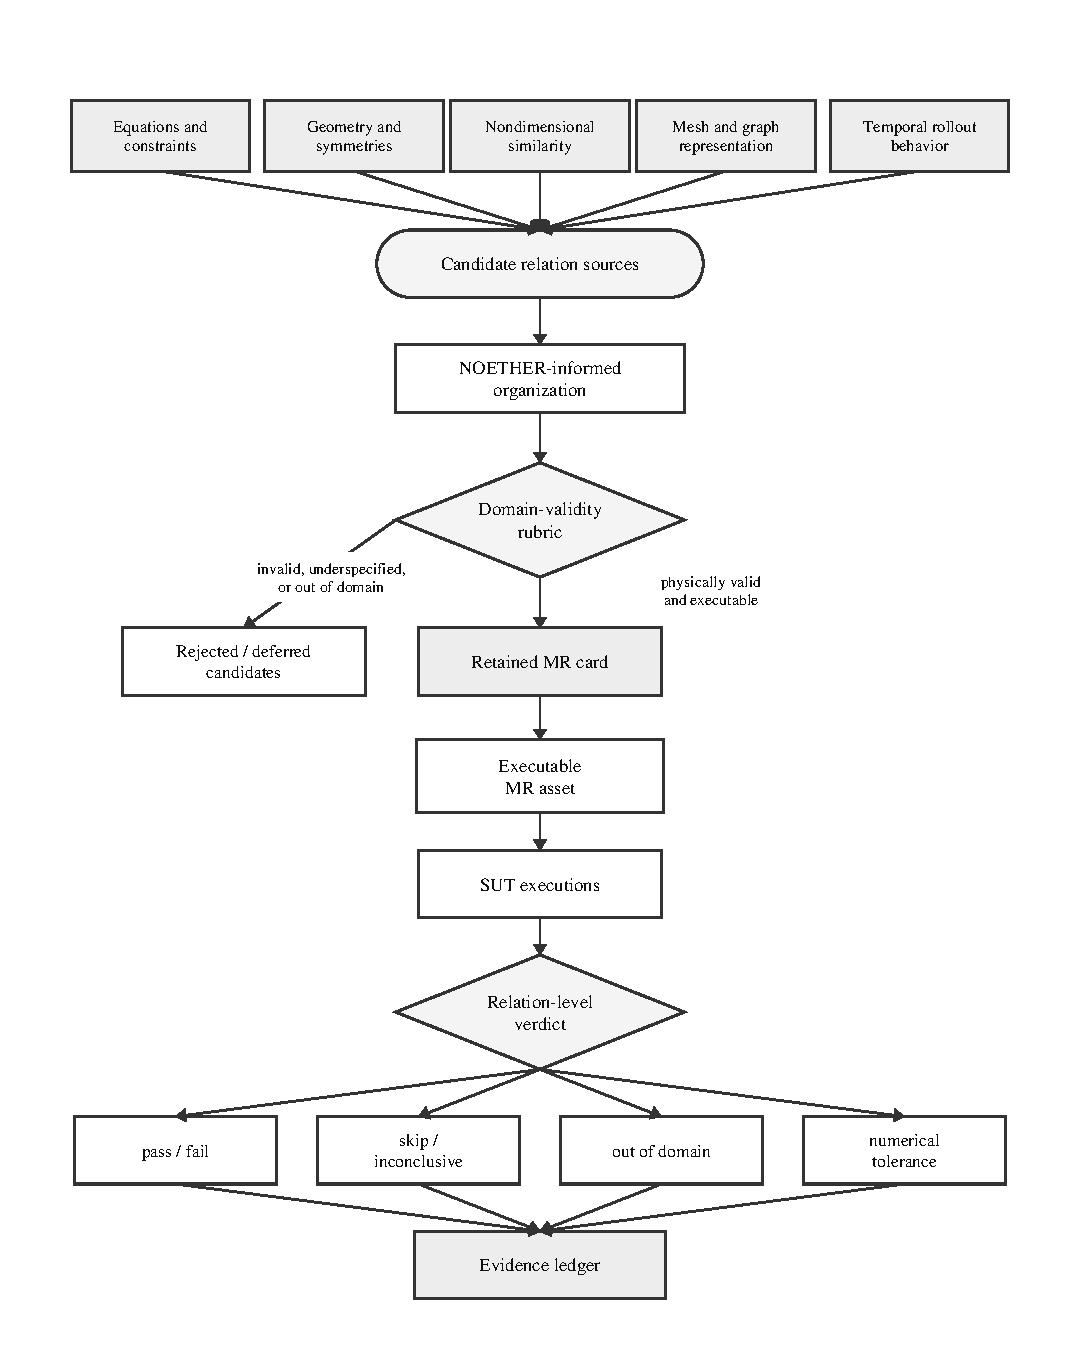
\includegraphics[width=0.85\linewidth]{figures/fig_1_validity_gated_workflow.pdf}
\caption{Validity-gated V\&V workflow.}
\label{fig:workflow}
\end{figure}

\subsection{Candidate relation sources and relation families}
\label{subsec:candidate-sources}

Candidate relations can come from physical laws, dimensional reasoning, expert knowledge, prior metamorphic-relation identification for scientific software, and large language model-assisted lists; a same-author preprint also catalogs physics-derived candidate relations for this surrogate class \citep{li2026noether}, superseding an earlier descriptive physical/computational/code classification \citep{yang2020hierarchical}. How a candidate is sourced does not affect its admissibility: the central decision point is the gate of Section~\ref{subsec:rubric}, which applies to any candidate. To keep the case studies organized, we group candidate relations into \emph{families} by the invariant each one encodes, and name each family by that invariant rather than by any particular transformation.

Several families are referenced in this paper. A \emph{reflection-symmetry} (equivariance) family asks that the surrogate commute with a spatial reflection; its cylinder-flow instance is mirror-y reflection. A \emph{conservation} family asks that a conserved quantity be preserved; its instances are discrete-divergence continuity for cylinder flow and compressible mass balance for the airfoil task. A \emph{representation-invariance} family asks that the output be invariant to a relabeling of the mesh; its instance is node-permutation equivariance and the encoding contract. A \emph{convergence/accuracy-order} family asks that a discrete operator approach its continuum limit at the expected rate; its instance is the operator-floor mesh-refinement relation. A \emph{monotonicity} family (Reynolds--Strouhal ordering) is a candidate not exercised here. Two further families, trajectory-reversal and self-adjointness, are not exercised in this paper's case studies; trajectory reversal in particular is empty by construction for viscous dissipative flow.

Grouping by invariant is an organizing convenience, not a validity argument. The same family may be admissible in one setting and inadmissible in another once instantiated for a specific surrogate: mirror symmetry holds on a symmetric domain but not on an asymmetric mesh with incompatible boundary labels, and conservation is a physical expectation but not an executable verdict when the discrete measuring operator has an unresolved error floor. The admissibility gate records where each relation survives.

\subsection{Admissibility gate}
\label{subsec:rubric}

A candidate relation is an \emph{admissible MR} only when four conditions hold together. First, (i)~it must have a physical or software basis. Second, (ii)~its transformation preconditions must hold for the source and follow-up cases. Third, (iii)~boundary conditions and output mappings must remain compatible after transformation. Fourth, (iv)~the verdict must be numerically decidable: the tolerance must dominate the intrinsic error floor of the measuring operator. None of these conditions is optional. Table~\ref{tab:rubric} records the gate, the MR-card fields, and the verdict semantics.

\begin{table}[H]
\centering
\caption{Admissibility gate and verdict semantics.}
\label{tab:rubric}
\footnotesize
\renewcommand{\arraystretch}{0.92}
\setlength{\tabcolsep}{3pt}
\begin{tabularx}{\textwidth}{@{}>{\raggedright\arraybackslash}p{0.18\textwidth}>{\raggedright\arraybackslash}p{0.31\textwidth}>{\raggedright\arraybackslash}p{0.29\textwidth}Y@{}}
\toprule
\textbf{Method element} & \textbf{Required record} & \textbf{Allowed interpretation} & \textbf{Design role} \\
\midrule
Basis & Equation, boundary condition, nondimensional law, representation property, numerical assumption, or implementation contract & Relation may be considered only for SUTs where this basis applies & Gate \\
Preconditions & Source-case constraints, follow-up transformation, preserved quantities, and exclusion rule & Missing preconditions produce skip or out-of-relation-domain, not SUT failure & Gate \\
Mapping compatibility & Boundary-label compatibility and output mapping from follow-up output back to source coordinates/fields & Incompatible mapping rejects or downgrades the candidate & Gate \\
Numerical decidability & Metric, tolerance, tolerance provenance, and measurement-floor evidence & A verdict is meaningful only when tolerance dominates the operator floor & Gate \\
MR card & Identifier, source category, transformation, mapping, metric, tolerance, exclusions, expected verdicts, and artifact schema & The admitted relation becomes a reusable executable V\&V asset & Asset \\
Evidence ledger & Source/follow-up run ids, metric outputs, floor evidence, exclusions, logs, and verdict & The reported claim is auditable from artifacts rather than prose alone & Asset \\
Verdict semantics & Pass, fail, skip, out-of-relation-domain, numerical-tolerance issue, or inconclusive & Only fail inside the valid domain may be read as SUT inconsistency & Verdict \\
\bottomrule
\end{tabularx}
\end{table}

The gate produces four design-time decisions: admit as an executable MR; downgrade to OOD-stress when the relation is physically informative but outside its exact domain; reject when basis, preconditions, or mapping fail; or defer when missing numerical evidence prevents a verdict. For example, node permutation can be admitted as a representation MR when the adapter and inverse mapping are deterministic; mirror-y is conditional on compatible geometry, boundary labels, and vector-component mapping; absolute discrete divergence is deferred when the reference field and measuring operator floor cannot support an absolute verdict.

\subsection{MR card and executable asset format}
\label{subsec:mr-card}

A retained MR is represented as a structured MR card recording the fields listed in Table~\ref{tab:rubric}: identifier, source category, physical or software basis, source-case schema, follow-up transformation, preconditions, boundary-condition compatibility, output mapping, metric, tolerance and provenance, expected verdict classes, exclusion rules, artifact schema, and interpretation limits. The card is the reusable design record; the executable runner is the operational artifact generated from it.

Each executable asset includes transformation code, runner configuration, metric computation, verdict logic, and artifact recording. The ledger is part of the method rather than only replication packaging: every relation-level claim must be traceable to the source run, follow-up run, mapping, metric output, floor evidence, exclusion decision, and verdict.

\subsection{Relation-level verdicts}
\label{subsec:verdicts}

An MR execution can produce: \textbf{pass} (relation holds within tolerance); \textbf{fail} (violated within the valid relation domain); \textbf{skip} (required precondition missing); \textbf{out-of-relation-domain} (the transformed case is outside the relation domain); \textbf{numerical-tolerance issue} (the measured effect is dominated by threshold or resolution uncertainty); or \textbf{inconclusive} (insufficient artifact).

These verdicts form the two-dimensional space in Figure~\ref{fig:verdict-2d}. One axis is relation-violation magnitude, typically expressed as a violation-to-floor or violation-to-tolerance ratio. The other is domain-violation magnitude: how far the transformed case lies outside the relation's validity domain. Low domain violation with high relation violation is the region that may be read as SUT inconsistency; high domain violation is out-of-relation-domain; a violation inside the error floor is a numerical-tolerance issue. This decomposition defines the method's verdict-interpretation role, which is evaluated explicitly in Section~\ref{subsec:rqs}.

In this study, the domain-violation coordinate is operationalized per relation from committed measurements. For mirror-y, $D = m/(m+1)$, where $m$ is the worst reflected-node placement error in median-edge-length units. The synthetic symmetric mesh scores $D \approx 0$, whereas the real asymmetric evaluation mesh scores $D = 0.51$. Other MR families use their own precondition measurements. These $D$ values denote structural placement within each relation's own validity domain: $D$ is a per-relation normalized coordinate, not a cross-relation calibrated metric, and the values cannot be averaged or ranked across MR families; read per relation, not as a calibrated boundary measurement. A cross-relation calibration would need to normalize each family by its own admissibility boundary, mapping every gate threshold to a common $D_{\mathrm{cal}} = 1$; that calibration is future work.

\begin{figure}[!htbp]
\centering
\makebox[\linewidth][c]{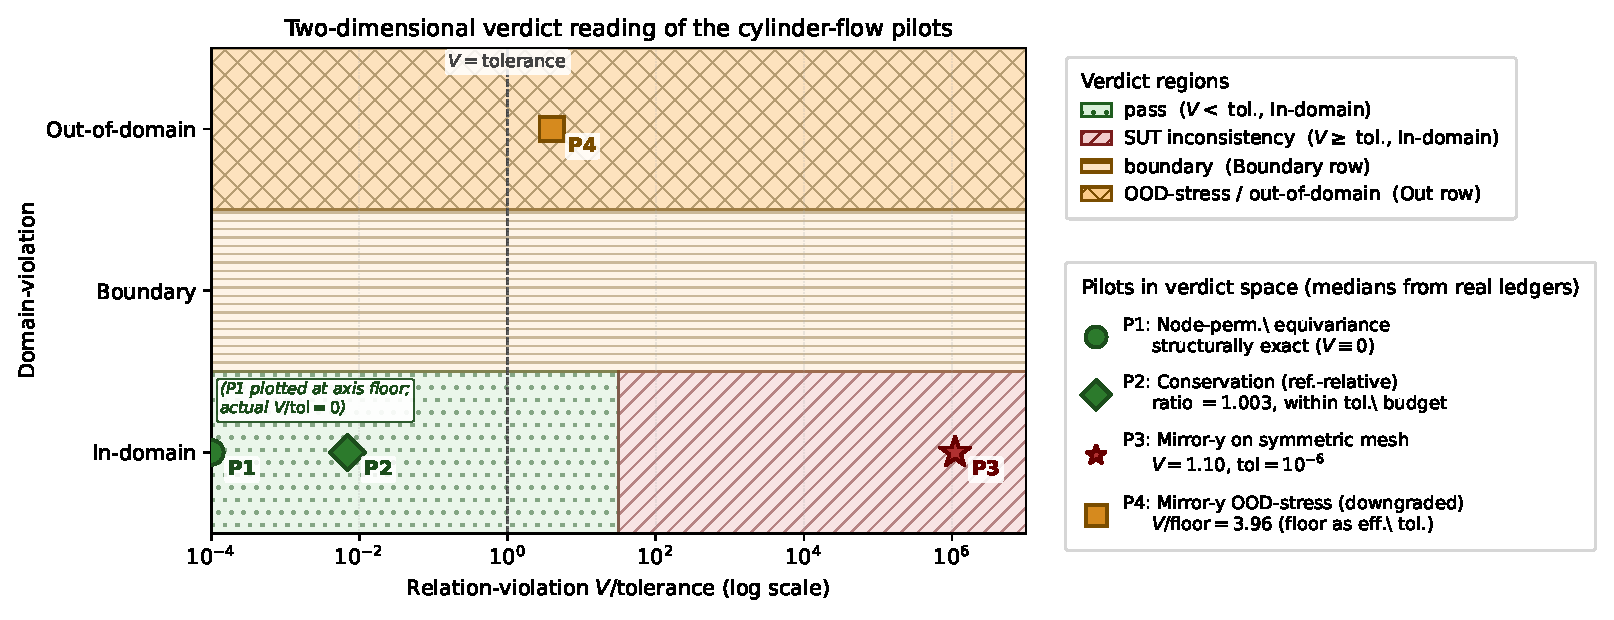
\includegraphics[width=1.08\linewidth]{figures/fig_3_verdict_2d.pdf}}
\caption{Two-dimensional relation and domain verdict space.}
\label{fig:verdict-2d}
\end{figure}

Retained relations are interpreted through the invariant each family encodes (Sec.~\ref{subsec:candidate-sources}): the invariant a relation measures fixes which faults it can and cannot surface. This is an interpretation protocol, not a validated localization model; the seeded-fault results later are a bounded stress test of it.

\section{Experimental Design}
\label{sec:empirical-design}

\subsection{Research questions}
\label{subsec:rqs}
\label{subsec:evaluation-logic}

The experimental design is organized around the following objective: to evaluate whether physics-derived MRs for SciML surrogate software can be transformed into auditable, executable, and interpretable oracle-free V\&V assets that distinguish genuine SUT inconsistency from relation invalidity and numerical measurement limits.

This objective is decomposed into four research questions:
\begin{description}[leftmargin=!,labelwidth=2.4cm]
\item[RQ1 -- Admissibility.] What validity conditions determine whether a physics-derived candidate MR is admissible as an oracle-free test for a specific SciML surrogate SUT?
\item[RQ2 -- Asset construction.] How can admissible MRs be represented as reusable MR cards and executable test assets with explicit transformations, mappings, metrics, tolerances, exclusions, and evidence records?
\item[RQ3 -- Verdict interpretation.] How can relation-level verdicts separate SUT inconsistency from out-of-relation-domain application, numerical tolerance limits, and inconclusive evidence?
\item[RQ4 -- Empirical utility.] In bounded SciML surrogate case studies, what evidence does the validity-gated workflow provide beyond rollout accuracy, generic MR generation, and LLM-assisted candidate elicitation?
\end{description}

\subsection{Experimental subjects}
\label{subsec:suts}

The subjects are selected for evidence roles rather than for statistical representativeness. A subject is included only when it contributes at least one design need: a primary end-to-end SciML surrogate setting with executable MR assets; a changed physical task or architecture that can falsify a checklist-only reading of the gate; a cross-family PDE/neural-operator setting that exercises the same admissibility predicate; or a bounded defect/coverage witness that ties MR responses to committed fault or true-fault-class evidence. The study does not select subjects by repository popularity, lines of code, or issue/changelog-mined defects; those criteria would require a separate real-defect study. The evidence below therefore supports bounded V\&V utility and coverage interpretation, not population-wide defect-detection effectiveness.

In aggregate, the executable subject inventory comprises one primary CFD task, one second CFD task, same-task MGN variants, one PointMLP SUT, PhysicsNeMo executions, PINN and FNO rosters over two PDEs, and five external central-processing-unit (CPU)-only SUT replays (Table~\ref{tab:subject-scope}). The fault-evidence inventory comprises 10 canonical MGN mutants, two adversarial MGN mutants, 48 PINN/FNO output-level probes, a PointMLP 20-fault catalog, and the external sibling's 70 witness rows and 20 true-fault-class rows. These counts are denominators for evidence scope; they are not sampling frames for a general defect-detection rate.

\begin{table}[!htbp]
\centering
\caption{Subject selection and evidence scope.}
\label{tab:subject-scope}
\scriptsize
\renewcommand{\arraystretch}{0.9}
\setlength{\tabcolsep}{2pt}
\begin{tabularx}{\linewidth}{@{}>{\raggedright\arraybackslash}p{0.17\linewidth}>{\raggedright\arraybackslash}p{0.36\linewidth}>{\raggedright\arraybackslash}p{0.24\linewidth}Y@{}}
\toprule
\textbf{Evidence block} & \textbf{Selection principle, subjects, and scale} & \textbf{Fault or defect evidence} & \textbf{Boundary} \\
\midrule
Cylinder-flow mesh surrogates & Primary executable workflow and same-task implementation variation: DeepMind \texttt{cylinder\_flow}; one pilot MGN checkpoint; K=6 checkpoint roster over three held-out trajectories; S4/S5 MGN variants; PointMLP; NVIDIA PhysicsNeMo \texttt{MeshGraphNet} smoke workflow & 10 canonical MGN mutants, two adversarial MGN mutants, and a PointMLP 20-fault catalog & Same task and bounded rosters; no real-defect rate or LOC-based representativeness \\
Airfoil mesh surrogate & Changed physics for gate discrimination: official DeepMind airfoil data; PhysicsNeMo \texttt{MeshGraphNet}; K=6 checkpoints over 40 test trajectories, producing 240 checkpoint--trajectory cells & Gate-rejected templates fire on the correct SUT, including mirror-y under non-zero angle of attack & Typed inadmissibility evidence, not state-of-the-art airfoil accuracy or official-checkpoint evidence \\
PINN and FNO PDE families & Cross-family admissibility predicate check: PINN with 15 Burgers and 15 heat seeds; FNO with six trained FNO-2D checkpoints plus a K=15-per-PDE admissibility roster & Unified catalog includes 24 closed-form PINN probes and 24 closed-form FNO probes & Output-level probes and trained rosters are breadth evidence, not real-defect corpora \\
External sibling programs & Independent breadth and true-fault-class witness: Minimum-MR-SubSet audit across seven program types; five CPU-only end-to-end SUT replays, including OpenMC & 70 real witness rows, 20 true-fault-class rows, and three SciML/PDE \texttt{PASS\_WITNESS} rows; sibling seeded-mutant kill matrices & Read-only/sibling provenance; no new issue/changelog mining in this paper \\
\bottomrule
\end{tabularx}
\end{table}

\emph{Primary evidence} comes from a MeshGraphNets-family cylinder-flow case study: a trained checkpoint, its six-checkpoint roster (K=6, with S0 denoting the pilot checkpoint), two same-domain wider/deeper variants (S4/S5), a PointMLP coordinate network, and the NVIDIA PhysicsNeMo \texttt{MeshGraphNet} production implementation evaluated on official DeepMind cylinder\_flow TensorFlow record (TFRecord) files. The primary unit is a relation-level cell: MR card, SUT/checkpoint, trajectory or source case, transformed follow-up case, metric, and verdict.

\emph{Supporting evidence} checks whether the same admissibility predicate applies outside the primary mesh-surrogate setting: a fifteen-seed PINN roster (K=15) and trained FNO-2D checkpoints over 2D Burgers and heat data.

\emph{Secondary evidence} includes LLM-simulated expert MR design, generic MR-generation scope contrasts, LLM-assisted candidate generation, rollout-accuracy diagnostics, and external witness reruns from the read-only Minimum-MR-SubSet repository.

\emph{Stress-test evidence} uses seeded-fault and cross-program checks to interpret where the admitted MR set can and cannot observe faults.

\subsection{Evaluation metrics}
\label{subsec:metrics}

Primary metrics are admissibility decision, executable MR rate, verdict distribution, violation magnitude relative to tolerance or floor, exclusion rate, and relation-level interpretation output. Secondary metrics include inter-rater agreement for candidate screening, flakiness rate, complementarity with rollout accuracy, and stress-test detection by seeded-fault class. These metrics are interpreted at the relation-cell level rather than as general reliability or defect-detection rates.

\subsection{Experimental method}
\label{subsec:experimental-method}

The experiments instantiate the candidate-to-asset workflow of Section~\ref{sec:method}. The relations evaluated are the cylinder-flow families of Section~\ref{subsec:candidate-sources}: reflection-symmetry (mirror-y) and conservation (discrete-divergence continuity), representation-invariance (node-permutation), and the convergence/accuracy-order pair (operator-floor refinement); the monotonicity and self-adjoint families are exercised only as candidate or cross-family checks, and trajectory-reversal is empty by construction. For each retained relation, the workflow records an MR card, source and follow-up executions, transformation and mapping artifacts, metric outputs, floor evidence, exclusions, and a typed verdict. The design separates four evidence tiers: primary, supporting, secondary, and stress-test evidence.

\subsection{Comparison baselines}
\label{subsec:baselines}

Rollout accuracy, residual/UQ diagnostics, expert-designed candidates, generic MR generators, and LLM-assisted candidates contextualize RQ4. Rollout accuracy asks whether a prediction is close to observed held-out data; an MR asks whether a declared relation holds under a controlled transformation. The baseline contrast is therefore complementarity and gate value: false-alarm removal, typed triage, auditability, and executable-asset reuse, not superiority in a shared scalar score. LLM and generic MR outputs are treated as candidate sources; the admissibility gate, not the generator, decides whether a candidate becomes an executable MR.

\subsection{Analysis plan and evidence mapping}
\label{subsec:rq-evidence}

Table~\ref{tab:rqmap} maps research questions to evaluation evidence, artifacts, units of analysis, and claim boundaries; it is a design rather than a result table.

\begin{table}[H]
\centering
\caption{Evaluation design.}
\label{tab:rqmap}
\scriptsize
\setlength{\tabcolsep}{1.5pt}
\begin{tabularx}{\linewidth}{@{}>{\raggedright\arraybackslash}p{0.08\linewidth}>{\raggedright\arraybackslash}p{0.22\linewidth}>{\raggedright\arraybackslash}p{0.20\linewidth}>{\raggedright\arraybackslash}p{0.21\linewidth}Y@{}}
\toprule
\textbf{Item} & \textbf{Evaluation question} & \textbf{Evidence tier and unit} & \textbf{Artifacts} & \textbf{Claim boundary} \\
\midrule
Goal & Does the full workflow connect candidate, gate, executable asset, verdict, and evidence? & Primary workflow trace; MR-card cell & MR cards, runners, claim ledger & Asset construction only; no general reliability claim \\
RQ1 & Which candidates are admissible, rejected, downgraded, or deferred? & Primary and supporting gates; candidate/MR & Rubric records, operator-floor sweep, exclusions & Physical validity is relation- and SUT-specific \\
RQ2 & Are admitted relations executable and auditable? & Primary execution cells; source/follow-up pair & Transformations, runner configs, metric files, logs & Execution completeness, not complete automation of MR discovery \\
RQ3 & Do verdicts separate SUT inconsistency from domain and numerical limits? & Verdict ledger; MR-by-case cell & Two-axis verdicts, metric/floor ratios, exclusion logs & Per-relation interpretation; no cross-relation calibrated domain score \\
RQ4 & What evidence is added beyond rollout accuracy and candidate-generation comparators? & Primary, supporting, secondary, and stress-test tiers & Rollout diagnostics, LLM/generic baselines, witness reruns, seeded-fault ledgers & Complementarity and bounded utility; no baseline superiority \\
Impl. & What blind spots follow from the admitted MR set? & Stress-test tier; mutant/MR cell & Seeded-fault catalog and cross-SUT removal check & Bounded coverage interpretation, not real-world detection rate \\
\bottomrule
\end{tabularx}
\end{table}

The study reports inferential statistics only where the sampling structure supports them, labeling descriptive counts otherwise. Binary detector outcomes over the unified fault catalog carry Wilson 95\% confidence intervals (CIs) per detector; continuous violation magnitudes use exact Wilcoxon signed-rank tests with a rank-based effect size (Cliff's $\delta$), where the design supports paired comparison; roster medians carry paired bootstrap intervals; and the operator-floor sweep reports a log-log slope with a 95\% CI. Repeated cells from one trajectory or one checkpoint family are reported as descriptive cell summaries, not independent population samples.

\subsection{Ethics, integrity, and reproducibility}
\label{subsec:ethics}

The study does not involve human subjects or personal data. SUT versions, datasets, checkpoints, scripts, and run logs are recorded when licensing permits. Failed, skipped, out-of-relation-domain, numerical-tolerance, and inconclusive outcomes remain in the ledger. LLM use is restricted to candidate generation and evidence organization, not validity judgment. No candidate MR is described as valid without a passing gate decision and MR card; no OOD violation is described as a program fault without supporting verdict evidence.

\section{Results and Discussion}
\label{sec:results}

Evidence is reported by research question rather than execution chronology, following the RQ-to-evidence mapping of Table~\ref{tab:rqmap}. The cylinder-flow case study is the primary evidence; the airfoil, PINN, FNO, and cross-program runs are supporting or secondary; fault-detection and cross-SUT coverage are discussed only as a bounded implication of the admitted MR set. Where a baseline contrast is reported (Appendix~\ref{app:secondary}), it measures the admissibility gate's own value rather than ranking methods: on the correct SUT a gate-admitted detector raises no false alarm while every gate-rejected template does, and against a rollout-accuracy monitor the MR suite is complementary, not superior. The secondary baselines, the external-scope audit, and the cross-family PINN and FNO executions that test whether the admissibility predicate is family-agnostic are reported in Appendix~\ref{app:secondary}.

\subsection{Evidence overview}
\label{subsec:claim-evidence-map}

The compact claim-to-evidence map binds every claim to a tracked artifact using reviewer-facing claim names; the full table is in Appendix~\ref{app:claim-evidence} (Table~\ref{tab:claim-evidence}), and the authoritative runtime mapping remains in \texttt{claim-ledger.yml}.

\label{subsec:mr-card-verdict-map}

Table~\ref{tab:mr-card-verdict} maps each retained MR card to its rubric decision, runtime verdict, and the interpretation boundary that verdict licenses.

{
\small
\renewcommand{\arraystretch}{0.96}
\setlength{\tabcolsep}{3pt}
\begin{xltabular}{\linewidth}{@{}>{\raggedright\arraybackslash}p{0.20\linewidth}>{\raggedright\arraybackslash}p{0.22\linewidth}>{\raggedright\arraybackslash}p{0.22\linewidth}Y@{}}
\caption{MR-card verdict map.}\label{tab:mr-card-verdict}\\
\toprule
\textbf{MR card} & \textbf{Rubric decision} & \textbf{Runtime verdict} & \textbf{Interpretation boundary} \\
\midrule
\endfirsthead
\toprule
\textbf{MR card} & \textbf{Rubric decision} & \textbf{Runtime verdict} & \textbf{Interpretation boundary} \\
\midrule
\endhead
\bottomrule
\endlastfoot
Node permutation equivariance & Retained as representation MR & pass sanity; relative L2 = 0.0 & Supports one executable representation path; does not establish model reliability. \\
Mirror-y equivariance (asymmetric eval mesh) & Exact relation out-of-relation-domain; downgraded to approximate OOD-stress & S0 pilot: 10/10 fail; primary upgrade: 180/180 fail across K=6 x 3 trajectories x 10 & Bounded within-family OOD-stress violation across held-out trajectories; not by itself exact symmetry, cross-SUT, or geometry-independent evidence. \\
Mirror-y equivariance (synthetic symmetric mesh) & Exact relation admissible (bijection verified, offset $<10^{-12}$, type-match 1.0) & S0 pilot: fail, rel L2 1.10; primary upgrade: 18/18 fail across K=6 x 3 input seeds & Exact-symmetry failure where the relation is admissible; synthetic no-obstacle OOD meshes, not accuracy or cross-SUT evidence. \\
Discrete divergence / conservation & Absolute mass-conservation MR deferred; reference-relative diagnostic retained & S0 pilot inconclusive: reference-relative non-regression guard; primary upgrade: 162/162 pass across K=6 x 3 trajectories x 9 & Reference-relative diagnostic only; the absolute conservation relation remains deferred. \\
MGN S4/S5 variant workflow & Node permutation admitted; mirror OOD/\allowbreak conservation diagnostic/exact-symmetry decisions recorded & 2/2 node-permutation passes; 60/60 mirror OOD failures; 54/54 conservation-diagnostic passes; 6/6 exact-symmetry failures & Same-domain MGN variant evidence, not an external SUT family. \\
PointMLP cylinder workflow & Node permutation admitted; mirror OOD/\allowbreak conservation diagnostic/exact-symmetry decisions recorded & 9/9 node-permutation passes; 10/10 mirror OOD failures; 9/9 conservation-diagnostic passes; 3/3 exact-symmetry failures & Different non-MGN cylinder SUT; not PhysicsNeMo/EchoWave or production CFD evidence. \\
PhysicsNeMo MGN Object-A smoke workflow & Node permutation admitted; mirror OOD/\allowbreak conservation diagnostic decisions recorded & Node permutation passes on the smoke subset (relative L2 0.0); rollout, mirror OOD, and conservation diagnostic ledgers recorded & Production-framework artifact-chain smoke evidence only; no full-scale production pass/fail rate and not external-aerodynamics evidence. \\
FNO periodic translation and conservation & Translation admitted; periodic discrete-conservation MR admitted-with-reference-floor; Dirichlet translation rejected & FNO primary workflow upgrade: 24/24 translation passes, 24/24 conservation failures, and 6/6 rejected Dirichlet exact-MR executions & Full rubric-to-verdict FNO evidence with raw source/follow-up outputs and per-case ledgers; outside cylinder-flow and broad neural-operator claims. \\
\end{xltabular}
}

\subsection{Primary cylinder-flow evidence}
\label{subsec:within-sut-pilot}

All pilots run on one real trained MeshGraphNets cylinder-flow surrogate, using the read-only Minimum-MR-SubSet checkpoint recorded in the experiment ledger. They exercise three different rubric outcomes; raw outputs, manifests, and metric ledgers are committed (Table~\ref{tab:claim-evidence}).

Table~\ref{tab:primary-result-summary} gives a compact reading guide for the detailed evidence that follows. It is not a separate analysis; each row points to a relation-level result, its licensed interpretation, and the boundary that prevents overclaiming.

\begin{table}[!htbp]
\centering
\caption{Primary result summary.}
\label{tab:primary-result-summary}
\scriptsize
\renewcommand{\arraystretch}{0.95}
\begin{tabularx}{\linewidth}{@{}>{\raggedright\arraybackslash}p{0.19\linewidth}>{\raggedright\arraybackslash}p{0.23\linewidth}>{\raggedright\arraybackslash}p{0.25\linewidth}Y@{}}
\toprule
\textbf{Check} & \textbf{Observed result} & \textbf{Interpretation} & \textbf{Boundary} \\
\midrule
Node permutation & Relative L2 = 0.0 & Execution and inverse-mapping sanity check for a representation MR & Does not establish model accuracy or reliability \\
Asymmetric mirror-y & 10/10 OOD-stress failures; median relative L2 0.737 & The gate downgrades exact symmetry to stress evidence on this mesh & Not an exact symmetry verdict or geometry-independent fault claim \\
Continuity & Absolute conservation deferred; reference-relative ratio about 0.4--0.8\% & Numerical floor blocks an absolute verdict while allowing a non-regression diagnostic & Not an absolute mass-conservation claim \\
Rollout contrast & One-step median relative L2 0.0216; mirror-y violation about 34x larger & MR evidence answers a relation question distinct from accuracy & The quantities are different relative-L2 objects \\
Symmetric mesh & Exact mirror-y admitted and fails; relative L2 1.10 & The out-of-sample gate admits the relation when geometry is bijective & Synthetic no-obstacle OOD geometry \\
Seeded faults & 5/10 mutants detected; detections separate by MR family & Admitted MRs expose some invariant-breaking faults and blind spots & Stress-test evidence, not a real-world defect-detection rate \\
\bottomrule
\end{tabularx}
\end{table}

\textbf{Representation MR.} Node-permutation equivariance holds to machine precision (relative L2 = 0.0 at tolerance 1e-6). This is a structural property of message-passing and is reported as a pipeline-implementation sanity check rather than model capability or accuracy evidence.

\textbf{Geometric MR.} The rubric classifies exact mirror-y equivariance as out-of-relation-domain for this mesh (the reflection is non-bijective, the worst reflected-node mismatch is about one edge length, and the cylinder is off-center by 7.2 mm) and downgrades it to an approximate nearest-neighbor OOD-stress probe scored against a same-space mapping-error floor. The probe failed on 10 of 10 recorded eval frames (median relative L2 0.737, median V/floor 3.96, floor range 3.02--5.55x), with no frame skipped or inconclusive. This is a bounded within-SUT frame-level OOD-stress result: one SUT, one checkpoint, one MR, one eval trajectory. The frames are consecutive, not independent samples, so the exact binomial 95\% interval for 10/10 is wide ([0.69, 1.00]). The mapping-error floor derives from the same geometric mismatch that triggered the downgrade, so V/floor alone cannot separate a model-level violation from an amplified geometric artifact on this mesh. The symmetric-mesh run below resolves that ambiguity.

\textbf{Continuity MR.} A piecewise-linear (P1) discrete-divergence operator produces a non-negligible divergence even for the ground-truth field on this coarse mesh, so an absolute divergence-free tolerance is not calibratable and the absolute mass-conservation relation stays deferred. As a reference-relative diagnostic, the surrogate's predicted next-state divergence stays within about 0.4--0.8\% of the reference on the recorded eval frames; the interior-only ratio rules out a pure boundary-imposition artifact. This asserts no absolute conservation. Two caveats bound the diagnostic. First, the reference divergence is not yet decomposed into discrete-operator error, solver projection artifact, or genuinely non-solenoidal training data, so if the reference field is itself materially non-solenoidal the reference-relative ratio is a non-regression guard rather than a conservation measurement. Second, the diagnostic uses a 50\% regression threshold (ratio $>1.5$) on two eval frames only, so ``passes'' means ``does not regress conservation by more than 50\% on those frames,'' not ``conserves mass.''

\textbf{Rollout-accuracy diagnostic.} On the same eval trajectory, the surrogate's one-step next-state prediction error ($v_\mathrm{pred}=v_t+$ denormalized predicted delta, the trainer's own convention) has median relative L2 0.0216 (mean 0.044; min 0.0116, max 0.0788) over the nine recorded transitions. The per-transition error is bimodal, so we quote both statistics. The mirror-y OOD-stress violation (median 0.737) is about 34 times the median accuracy and 17x the mean. The quantities are dimensionless relative L2 values of different objects, so this is an order-of-magnitude gap rather than a precise factor; it is one-step, not a free-running rollout-stability result.

\textbf{Exact mirror-y on a symmetric mesh.} We built a provably symmetric synthetic structured channel mesh whose reflection is a verified bijection (node-type match 1.0, reflection offset $<10^{-12}$, edge set invariant), so the predicate admits exact mirror-y. On one constructed input the surrogate fails this exact equivariance test (relative L2 1.10). The normalizer control changes the violation only from 1.1032 to 1.1014, so the violation is dominated by learned message-passing weights. The boundary is synthetic, no-obstacle OOD geometry: the result confirms missing exact equivariance but is not a calibrated in-distribution magnitude.

\textbf{Seeded-fault detection.} We re-implemented, from the read-only Minimum-MR-SubSet witness taxonomy, an injected-fault catalog of 10 pipeline faults across five fault classes (boundary-condition, mesh-adjacency, normalization-scale, temporal-rollout, physical-channel), and used the paper's own MRs as detectors on the model's predicted update. The continuity MR detected the two boundary-condition faults and the gross normalization fault (divergence ratio 3.8--10.6 vs the 1.5 threshold); the symmetry MR detected a physical-channel and a mesh-adjacency fault (violation rising 69--142\% above baseline); node-permutation equivariance detected none, because these faults preserve node-relabeling invariance. 5 of 10 mutants were detected by at least one MR, and the detections separate by MR family (continuity to boundary/scale faults, symmetry to physical-channel/adjacency faults), a first bounded test of the interpretation protocol of Section~\ref{subsec:verdicts}, suggestive rather than a validation. Three boundaries: the detected faults are gross corruptions that any divergence- or symmetry-sensitive detector would catch; the edge-drop fault is a near-miss (32\% mirror-y change vs the 50\% threshold) and the boundary faults are invisible to mirror-y by construction; and the remaining undetected faults shift the absolute output without crossing the scored-quantity thresholds, delimiting where these MRs are structurally insensitive. Against a rollout-accuracy monitor on the same faults the two are complementary: the edge-permutation and channel-swap faults the symmetry MR catches leave the rollout error within 1.3$\times$ of its in-distribution baseline (0.0216, under a 2$\times$ regression threshold), so the MRs surface relation violations an accuracy monitor leaves within band, while the gross boundary/normalization faults trip both and no fault is caught by accuracy alone (claim~C38). It is one SUT, one checkpoint, one injected-fault catalog.

The remaining subsections carry the same evidence at larger scope: the MGN roster tests denominator robustness, the operator-floor sweep calibrates numerical decidability, and the fault catalog bounds detector geometry. Whether the gate transfers beyond the original MeshGraphNets workflow is tested by the cross-family PINN and FNO executions reported in Appendix~\ref{app:secondary}.

\subsection{Method transfer across architectures and equations}
\label{subsec:method-transfer}

Before the detailed scope upgrades, this subsection foregrounds the evidence that the workflow is not tied to the single cylinder-flow checkpoint. The same four-condition admissibility predicate, applied unchanged, produces typed decisions across a wider and deeper MGN variant, a non-message-passing PointMLP, a production framework, a second governing equation (compressible airfoil flow), and a different model family (PINNs and FNOs). Table~\ref{tab:method-transfer} consolidates these settings; each row is an already-committed run detailed in the subsection or appendix it points to, not a new result.

\begin{table}[!htbp]
\centering
\caption{The same admissibility predicate applied unchanged across architectures and governing equations. Each row is a committed run detailed in the referenced subsection or appendix.}
\label{tab:method-transfer}
\scriptsize
\renewcommand{\arraystretch}{0.95}
\begin{tabularx}{\linewidth}{@{}>{\raggedright\arraybackslash}p{0.19\linewidth}>{\raggedright\arraybackslash}p{0.20\linewidth}>{\raggedright\arraybackslash}p{0.30\linewidth}Y@{}}
\toprule
\textbf{Setting} & \textbf{Architecture / equation change} & \textbf{Typed decision under the unchanged predicate} & \textbf{Detail; boundary} \\
\midrule
Cylinder-flow MeshGraphNets & one trained checkpoint, incompressible Navier--Stokes & node-permutation pass; mirror-y downgraded to OOD stress and fails; conservation deferred with reference-relative pass; exact symmetry admitted and fails & Sec.~\ref{subsec:within-sut-pilot}; primary quantitative anchor \\
MGN S4/S5 variant & same task, wider/deeper network & 2/2 node-permutation pass, 60/60 mirror OOD fail, 54/54 conservation pass, 6/6 exact-symmetry fail & Sec.~\ref{subsec:multicheckpoint-replication}; same architecture family, not a rate \\
PointMLP coordinate network & different architecture class, no message passing & 9/9 node-permutation pass, 10/10 mirror OOD fail, 9/9 conservation pass, 3/3 exact-symmetry fail & Sec.~\ref{subsec:multicheckpoint-replication}; non-MGN SUT, not a rate \\
PhysicsNeMo \texttt{MeshGraphNet} & production framework & node-permutation pass; mirror-y OOD fail & Sec.~\ref{subsec:multicheckpoint-replication}; production smoke, not a rate \\
Compressible airfoil (MGN) & different governing equations & node-permutation admitted and exact (240/240); incompressible continuity rejected on physical basis; mirror-y rejected on boundary precondition; compressible conservation deferred & Sec.~\ref{subsec:second-task}; gate discriminates by equation, primary-scale \\
PINN / FNO (Burgers, heat) & different model family and equations & family-agnostic typed verdicts: FNO periodic translation 24/24 pass and periodic conservation 24/24 fail; PINN reference-relative conservation 30/30 pass & App.~\ref{subsec:pinn-extension}; cross-family probe, not calibrated coverage \\
\bottomrule
\end{tabularx}
\end{table}

These settings show the same predicate produces typed decisions across architectures and equations on bounded subjects; they are supporting breadth, not a cross-SUT or geometry-independent pass/fail rate. The primary quantitative evidence remains within one MeshGraphNets checkpoint (Section~\ref{subsec:within-sut-pilot}). The subsections and appendix referenced in the table carry the per-run detail.

\subsection{Same-task replication}
\label{subsec:multicheckpoint-replication}

The single-checkpoint evidence is replayed on a K=6 MeshGraphNets roster and three official DeepMind held-out test trajectories from the Minimum-MR-SubSet loader. S0 reuses the pilot checkpoint, so this is a replication/variant check rather than six independent SUTs. Node permutation is exact on all checkpoints. The primary empirical scope upgrade gives a K=6 x 3 trajectories x 10 mirror-y OOD-stress grid with 180/180 failures, a K=6 x 3 trajectories x 9 conservation-transition grid with 162/162 reference-relative passes while absolute conservation remains deferred, and a K=6 x 3 exact-symmetric-mesh input grid with 18/18 failures. The upgrade removes the single-source-trajectory denominator while remaining within one architecture family and dataset, so per-cell counts are descriptive summaries, not independent-trial inference, with the K=6 checkpoint roster as the effective independent unit.

\textbf{Same-task multi-architecture replication.} Three further cylinder-flow executions test whether the verdict pattern is an artifact of one implementation. A same-domain S4/S5 wider/deeper MeshGraphNet variant package reproduces the pattern (2/2 node-permutation passes, 60/60 mirror OOD failures, 54/54 conservation-diagnostic passes, 6/6 exact-symmetry failures). A newly trained PointMLP coordinate network (a different architecture class with no message passing) reproduces it as well (9/9 node-permutation passes, 10/10 mirror OOD failures, 9/9 conservation-diagnostic passes, 3/3 exact-symmetry failures, median rollout relative L2 0.0298). Third, the NVIDIA PhysicsNeMo \texttt{MeshGraphNet} production implementation, trained and evaluated on official DeepMind cylinder\_flow TFRecords, reproduces the node-permutation pass and the mirror-y OOD-stress failure within a production framework rather than a research codebase. The same admissibility predicate, applied unchanged, produced the same typed decisions on all three; this replicates the verdict pattern across architectures on one task and dataset, asserting no cross-dataset rate.

\subsection{Second-task gate discrimination: compressible airfoil flow}
\label{subsec:second-task}

A direct test of a domain-validity gate is whether it produces the correct \emph{different} verdict when the physics changes. We apply the identical four-condition predicate to a second CFD task on a second official dataset: the DeepMind \textbf{airfoil} benchmark (SU2-simulated compressible transonic flow, 5{,}233-node meshes with density, pressure, and velocity), distinct from incompressible cylinder flow in both physics and data. The same official PhysicsNeMo \texttt{MeshGraphNet} (2.33M-parameter official configuration: hidden width 128, 15 processor steps) is trained for 40 epochs on 100 official airfoil train trajectories (graphics-processing-unit (GPU)-trained to a converged final loss near 0.14) across a K=6 checkpoint roster and evaluated per-trajectory on 40 official test trajectories, producing 240 (checkpoint, trajectory) pairs. The predicate produces a \emph{different typed inadmissibility structure}, and the difference is the result. \textbf{Node-permutation equivariance is admitted and exact} (240/240, relative L2 0.0, training-independent representation contract). \textbf{Incompressible divergence-free continuity is rejected at the physical-basis gate} (condition i) because the density varies by a median factor of 2.13x across the field, so $\nabla\cdot u=0$ is physically false here, the same relation that on cylinder flow passes conditions (i)--(iii) and is only \emph{deferred} at condition (iv), so the gate assigns a categorically different verdict \emph{type} for the physically correct reason on each task. \textbf{Compressible unsteady mass conservation} $\partial_t\rho+\nabla\cdot(\rho u)=0$ is the physically-correct replacement, its absolute discrete form deferred (uncalibratable operator floor) and a reference-relative diagnostic recorded (median residual ratio 1.01 across the K=6 roster). \textbf{Mirror-y chord symmetry is rejected at the boundary-precondition gate} (condition iii) because the SU2 trajectories carry a non-zero angle of attack. The one-step rollout error remains high at this training budget (median relative L2 0.92, near the signal magnitude) and is reported only as a training-state diagnostic. None of the four typed verdicts depends on rollout quality. The admission rests on a representation contract; the rejections and deferral rest on physical and numerical reasoning that follows from the task's governing equations and discretization, not from the surrogate's outputs. This explains why the typed structure transfers and discriminates across tasks even on this converged model. This is a primary-scale second-task gate-discrimination result on the official MeshGraphNet architecture (240 checkpoint-by-trajectory cells), not an official-checkpoint or state-of-the-art-accuracy airfoil result.

\subsection{Operator-floor resolution sweep}
\label{subsec:operator-floor-sweep}

The P1 discrete-divergence sweep on symmetric meshes, over nine resolutions, gives slope 0.984 with 95\% CI $[0.975, 0.992]$ and R$^2=0.9999$, matching O(h) (Figure~\ref{fig:operator-floor}). The \emph{absolute} floor is also closed-form for the concrete deployed-scale mesh: since the operator is exact on affine fields and the reference field is divergence-free, the measured floor equals the geometry-weighted second-order Taylor remainder exactly. A leading-order predictor from the analytic Hessian matches the measured floor to within 0.5\% (1.337 vs 1.343), and a rigorous a-priori upper bound from the Hessian's global spectral norm dominates it at every resolution. The same floor reproduces on a genuinely different topology --- an unstructured Delaunay triangulation of a jittered grid (worst triangle angle about 14 degrees) over the same domain and reference field --- with log--log slope 0.983 (Student-t 95\% CI $[0.953, 1.014]$, R$^2=0.999$), a matched-resolution unstructured-over-structured floor ratio of 1.06 median and 1.33 maximum, so the numerical-decidability verdict does not flip between the two topologies. The gate thus rests on a derived floor, not an empirical estimate, for this mesh; the floor is empirically topology-stable across these two mesh families, while a general unstructured-mesh bound remains future work. This is why absolute conservation remains deferred while the reference-relative non-regression guard is reported. A classical flux-form finite-volume operator instead admits a fully executable conservation verdict (claim~C34, supporting artifact).

\begin{figure}[!htbp]
\centering
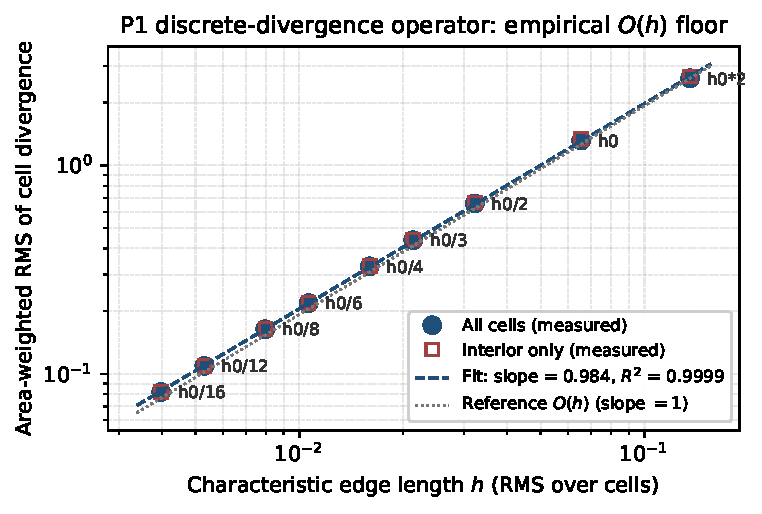
\includegraphics[width=0.82\linewidth]{figures/fig_4_operator_floor_loglog.pdf}
\caption{P1 divergence operator-floor calibration.}
\label{fig:operator-floor}
\end{figure}

\subsection{Coverage implication: fault-detection robustness across the multi-checkpoint roster}
\label{subsec:fault-robustness}

To check whether the primary MGN seeded-fault result of Section~\ref{subsec:within-sut-pilot} reproduces beyond one checkpoint and delimit where its detectors are structurally insensitive, the 10-mutant catalog is replayed against the K=6 multi-checkpoint roster across five input-permutation seeds (30 trials per mutant per detector), with two predeclared severity dimensions swept: NS\_double\_scale $s \in \{1.1, 1.25, 1.5, 2, 4\}$ and PC\_zero\_vy partial fraction $p \in \{0.25, 0.5, 0.75, 0.85, 0.9, 0.95, 0.99, 1.0\}$ (the canonical mutant is $p = 1.0$). Detection is decided by the same predeclared thresholds as Section~\ref{subsec:within-sut-pilot} (node-permutation tolerance $10^{-5}$, conservation ratio threshold 1.5, mirror-y relative-change threshold 0.5). Wilson 95\% CIs are computed across the (SUT, seed) cells; raw outputs are committed (Table~\ref{tab:claim-evidence}). This 10-mutant replay is the primary MGN stress-test denominator, not the whole fault-evidence inventory summarized in Section~\ref{subsec:suts}.

Table~\ref{tab:coverage-geometry} summarizes the coverage geometry that would otherwise be buried in several paragraphs. The table should be read by row: each admitted relation measures one invariant family, and the blind cells are therefore structural, not sampling noise.

\begin{table}[!htbp]
\centering
\caption{Coverage-geometry matrix.}
\label{tab:coverage-geometry}
\scriptsize
\renewcommand{\arraystretch}{0.93}
\begin{tabularx}{\linewidth}{@{}>{\raggedright\arraybackslash}p{0.18\linewidth}>{\raggedright\arraybackslash}p{0.26\linewidth}>{\raggedright\arraybackslash}p{0.26\linewidth}Y@{}}
\toprule
\textbf{Detector / relation family} & \textbf{Visible directions} & \textbf{Blind or excluded directions} & \textbf{Scope and boundary} \\
\midrule
Node permutation & Representation contract passes exactly; also admitted on airfoil & Canonical injected faults preserve node relabeling, so no mutant is detected & Sanity/adapter evidence, not fault-coverage evidence \\
Continuity / conservation & Boundary-condition faults and gross normalization faults; shared continuity $\to$ normalization-scale signal on airfoil & Multiplicative output scaling sweep remains undetected (0/6, CI $[0.00,0.39]$) & Measures conservation-like invariants only; absolute MGN conservation remains deferred \\
Mirror-y symmetry & Physical-channel and mesh-adjacency faults; partial $v_y$ zeroing detected through $p=0.99$ (6/6) & Exactly uniform $p=1.0$ is blind (0/6); mirror-y excluded on non-zero-angle airfoil & Coverage disappears when the relation is inadmissible \\
Admitted suite & 5/10 canonical MGN mutants detected; reproduces across S0--S3, with 4/10 on S4/S5 & Invariant-preserving faults remain invisible, including adversarial escapes & Bounded stress-test coverage, not real-world defect-detection rate \\
Cross-family / cross-program checks & PINN/FNO probes and sibling programs reproduce the invariant-based reading & Trained-mutant MGN/PointMLP evidence and closed-form PINN/FNO probes are not interchangeable & Breadth evidence only; no calibrated coverage law \\
\bottomrule
\end{tabularx}
\end{table}

\textbf{Aggregate reading.} The 5-of-10 union detection rate from C10 reproduces across S0--S3 and nearly across S4/S5. By-class localization also reproduces: continuity is sensitive to boundary/scale faults, whereas mirror-y is sensitive to physical-channel and adjacency faults. The severity sweeps in Table~\ref{tab:coverage-geometry} delimit the same point: faults are caught when they perturb a measured invariant and are invisible when they preserve all admitted invariants.

\textbf{Unified catalog and adversarial checks.} Phase 3 emits a 60-entry catalog (10 canonical MGN mutants, 2 adversarial MGN mutants, 24 closed-form PINN probes, and 24 closed-form FNO probes). Its descriptive precision/recall summary is node-permutation 1.00/1.00, conservation 1.00/0.81, and mirror-y 0.94/0.55; these rates summarize non-independent checkpoint-by-seed cells, not independent population items. The PINN/FNO probes further show a falsifiable blind region: faults preserving every measured invariant are detected by no relation, even when a transport fault corrupts the PINN field by 0.63 relative L2. The adversarial mutants test whether this blind region is a subspace: A1 leaves node permutation and conservation at 0/6, and A2 escapes every detector.

\textbf{Cross-SUT and cross-program breadth.} On the primary-scale PhysicsNeMo airfoil task, the gate excludes mirror-y because of non-zero angle of attack, and the mirror-only cylinder-flow coverage disappears; the shared continuity $\to$ normalization-scale signal remains. This supports the qualitative validity-coverage duality, but only at fault-class level on two CFD SUTs. The Minimum-MR-SubSet sibling adds an external breadth audit across seven program types and five CPU-only replays; Appendix~\ref{app:cross-program} gives the details.

\subsection{Interpretation and boundaries}
\label{sec:discussion}
\label{subsec:still-blocked}
\label{subsec:scoped-interpretation}

The value of the current study is not that every MR finds a new fault beyond rollout accuracy. Retained MRs provide relation-level evidence under explicit transformations; on a violation or deferral, the MR card and verdict rule help distinguish model inconsistency, relation-domain boundary, numerical tolerance issue, and inconclusive evidence.

Table~\ref{tab:interpretation-boundary} separates the interpretation licensed by the evidence from claims that remain outside scope.

\begin{table}[!htbp]
\centering
\caption{Interpretation and claim-boundary guide.}
\label{tab:interpretation-boundary}
\scriptsize
\renewcommand{\arraystretch}{0.93}
\begin{tabularx}{\linewidth}{@{}>{\raggedright\arraybackslash}p{0.20\linewidth}>{\raggedright\arraybackslash}p{0.26\linewidth}>{\raggedright\arraybackslash}p{0.25\linewidth}Y@{}}
\toprule
\textbf{Reader concern} & \textbf{Evidence response} & \textbf{Licensed claim} & \textbf{Not licensed} \\
\midrule
Does MR evidence add value beyond accuracy? & Rollout accuracy and mirror-y violation measure different objects; seeded faults include MR-only catches & Relation-indexed checks complement accuracy monitoring & MR suite superiority over accuracy monitors \\
Is the gate merely post-hoc labeling? & Symmetric-mesh, airfoil, PINN, FNO, and witness reruns apply the same predicate outside the first pilot & The predicate changes or preserves verdicts according to relation conditions & General reliability from one MeshGraphNets family \\
Does downgrading hide robustness failures? & OOD verdicts remain reported as stress or robustness evidence, but not as valid-domain fault verdicts & Gate controls fault attribution & Using domain invalidity to excuse deployment weakness \\
Is deferred conservation a pipeline failure? & FNO periodic conservation and PINN reference-relative conservation produce executable verdicts where the floor is calibratable & The gate fails closed when numerical decidability is missing & Absolute MGN mass conservation on the coarse mesh \\
What overclaims are blocked? & Typed verdicts distinguish failure, OOD stress, rejection, deferral, and inconclusive evidence & Bounded V\&V utility with auditable artifacts & Geometry-independent rates, validated localization, or real-world defect detection \\
When is the method worth using? & A relation must be physically meaningful and numerically decidable for the deployed discretization & Use for relation-indexed OOD or physics checks alongside accuracy/UQ & Replacement for residual, UQ, or accuracy diagnostics \\
What is the cost profile? & Card authoring and floor analysis are one-time per-relation design costs; runners then replay automatically & Reusable executable MR assets with visible assumptions & Zero-cost automatic MR discovery or measured person-hour savings \\
\bottomrule
\end{tabularx}
\end{table}

Two misreadings are especially important. First, without the gate, asymmetric-mesh mirror-y could be read as a model fault rather than an out-of-relation-domain stress result; with the gate, it remains a robustness signal but not a valid-domain defect oracle. Second, without the floor check, absolute discrete-divergence could be misread as a conservation pass despite reference-field divergence. The added runs answer whether this is only post-hoc labeling: the same predicate admits, rejects, or defers relations differently on symmetric meshes, airfoil, PINN, and FNO subjects, while preserving the stated reliability and geometry-independent-rate boundaries.

\textbf{Boundary of claims.}
\label{subsec:boundary-claims}

The canonical blocked list remains active: the evidence does not support external-dataset or geometry-independent pass/fail rates, AeroGraphNet/DoMINO results, comparative superiority over baselines, real-world fault-detection rates, validated localization, runtime, reliability, or model accuracy claims. The supported claim is that a domain-validity-aware workflow makes MR identification and execution more auditable for the studied class of SciML SUTs.

\textbf{Implications for SciML testing.}
\label{subsec:implications}

The scoped evidence shows how SciML testing can move from implicit expert checks to explicit MR assets that complement residuals, UQ, and accuracy by making transformations and verdict rules inspectable. The workflow targets a relation-indexed applicability map in relation space rather than residual space; calibrated maps across SUTs, trajectories, and domain-violation scores remain future work.

\textbf{When to use, and at what cost.} The gate earns its overhead when a surrogate must be trusted out of distribution and a physically necessary relation can be both stated for the task and made numerically decidable for the deployed discretization. Authoring an admissible MR requires domain knowledge to state the relation, numerical analysis to set or reject the floor, and testing expertise to bind transformations, mappings, metrics, and ledger fields. This paper decomposes those roles and provides reusable records and runners, but it does not measure person-hours, inter-author agreement, or maintenance cost; those are adoption questions for future work.

\section{Threats to Validity}
\label{sec:threats}

We classify threats following Verdecchia et al.~\citep{verdecchia2023threats} and report against the Empirical Standards for software engineering research~\citep{ralph2021empirical}.

\textbf{Construct validity.} The main construct is not ``model correctness'' but validity-gated MR asset construction. A wrong physical premise, boundary-condition reading, output mapping, discrete operator, or tolerance could therefore change an admit/reject/defer decision. We mitigate this by requiring an MR card, explicit preconditions, typed verdicts, and an operator-floor argument before a relation is treated as executable evidence. The mitigation is still incomplete: the P1 divergence floor is derived for the deployed symmetric-mesh setting and is empirically stable on a second unstructured Delaunay topology but is not proven for arbitrary unstructured meshes, and the reference-relative conservation diagnostic remains a non-regression guard rather than an absolute conservation measurement. The seeded-fault catalog also measures detector sensitivity to author-implemented mutants, so its rates do not estimate real-world defect prevalence or effectiveness. A gate verdict can prevent invalid fault attribution, but it must not be read as dismissing deployment robustness concerns outside the relation domain.

\textbf{Internal validity.} SUT setup, checkpoint selection, random seeds, mesh preprocessing, normalization, and runtime nondeterminism may affect verdicts. The study records manifests, ledgers, and raw outputs, and it repeats the primary cylinder-flow checks across K=6 checkpoints, three held-out trajectories, same-task variants, PointMLP, and PhysicsNeMo. These repetitions reduce the risk of a single-run artifact, but do not make the cells independent population samples. For airfoil, the surrogate is trained to convergence (40 epochs, final loss near 0.14) but its one-step eval rollout remains high (relative L2 0.92); its evidence is read for typed gate discrimination, not model accuracy.

\textbf{External validity.} The evidence covers incompressible cylinder flow, compressible airfoil flow, bounded PINN/FNO Burgers and heat executions, and a read-only/executed cross-program breadth check from the Minimum-MR-SubSet sibling artifacts. This shows the gate is not a one-off cylinder-flow checklist, but remains far from a general claim about SciML surrogates. Broader neural operators, mesh simulators, production CFD solvers, PINN architectures, datasets, geometries, and training regimes remain outside the evidence. The cross-program breadth check reuses the sibling's domain assets and mutant sets, so it supports only a qualitative coverage-geometry reading, not per-program reliability, new MR discovery, superiority, or real-world fault-detection rates.

\textbf{Baseline and comparator validity.} Rollout accuracy, residual/UQ-style diagnostics, generic MR templates, and LLM-assisted candidate generation are used as scope contrasts rather than defeated competitors. The LLM baselines depend on prompt design, model versions, and simulated raters; they show why an admissibility gate is needed, but are not a human-expert study and do not establish superiority over alternative MR-identification methods. The deterministic rubric, not LLM output, is the validity authority.

\textbf{Conclusion validity.} The study combines descriptive counts, Wilson intervals, bootstrap intervals, and exact nonparametric tests where the sampling unit supports them. Many reported cells share checkpoints, trajectories, or generated cases, so are not independent population trials. The primary MGN scope upgrade improves the weakest denominators within the stated scope, but the correct conclusion is bounded empirical utility for RQ4, not a calibrated reliability or coverage rate.

\textbf{Reproducibility.} Some workflows depend on old runtimes, public benchmark loaders, or non-redistributable checkpoints. The replication package therefore emphasizes scripts, manifests, run logs, claim ledgers, and available outputs. Reproducibility is strongest for artifact inspection and rerunnable CPU workflows, weaker for exact recreation of every trained checkpoint environment. By re-run cost: the operator-floor sweep, MR-card validators, and typed-verdict logic replay on CPU in minutes from committed scripts alone; the cylinder-flow MGN pilot, K=6 roster, PointMLP, and FNO/PINN rosters replay on CPU from committed checkpoints and metric ledgers; PhysicsNeMo MGN and airfoil training require a GPU and the public DeepMind TFRecords; and the Minimum-MR-SubSet audit and rerun execute read-only from sibling fixtures at the cited commit.

\section{Future Work}
\label{sec:future-work}

Future work should generalize the numerical admissibility gate beyond the deployed P1 symmetric-mesh setting to unstructured meshes, boundary treatments, and flux-form operators.

Second, the domain-violation axis should be calibrated across MR families. Here, domain distance is a per-relation interpretive coordinate, not a cross-MR score. A calibration protocol would normalize distances within relation families, define in-domain/near-boundary/out-of-relation-domain anchor cases, build relation-family calibration sets, and use independent experts or raters to validate categories, agreement, and residual comparability limits.

Third, the MR-card workflow should be evaluated on production-scale SUTs and datasets: external aerodynamics, production graph simulators, longer rollouts, and multi-physics pipelines.

Fourth, the coverage implication should be tested with independent real-defect corpora and independently authored mutants, asking whether admitted MR sets predict externally collected defect classes.

Finally, MR-card authoring, precondition checking, and ledger generation need automation and user studies of authoring effort, role division, inter-author agreement, and maintenance cost, while validity decisions remain tied to physical, numerical, and software evidence rather than model consensus.

\section{Conclusion}
\label{sec:conclusion}

This paper asked how physics-derived MRs for SciML surrogate software can be transformed into auditable, executable, and interpretable oracle-free V\&V assets. The answer is a validity-gated workflow: a candidate relation is first checked for physical basis, domain preconditions, representation mapping, and numerical decidability; admitted relations are recorded as MR cards and executable assets; and outcomes are interpreted with typed verdicts rather than a single pass/fail label.

The empirical evidence is bounded but artifact-backed. On cylinder-flow MeshGraphNets, the workflow separates a representation pass, an out-of-relation-domain mirror probe, a deferred absolute conservation relation, and a reference-relative diagnostic; the same readings are replayed across checkpoints, trajectories, and same-task architectures. On airfoil, PINN, and FNO subjects, the gate changes or preserves verdicts according to the relation's physical and numerical conditions. Seeded-fault stress tests further show that the admitted MR set helps explain detector blind spots in the studied settings, without implying general defect-detection rates or excusing OOD robustness failures.

The contribution is therefore methodological: physically meaningful SciML metamorphic tests require explicit validity conditions, executable assets, raw evidence records, and relation-level verdicts. This turns candidate MRs from informal expert intuitions into auditable V\&V assets with boundaries visible to reviewers and practitioners.

\section*{Preprint}
An earlier preprint version of this manuscript is available on arXiv at \url{https://arxiv.org/abs/2606.17529} with DOI \url{https://doi.org/10.48550/arXiv.2606.17529}.

\section*{CRediT authorship contribution statement}
\textbf{Meng Li:} Conceptualization, Methodology, Software, Writing -- original draft. \textbf{Xiaohua Yang:} Supervision, Formal analysis, Writing -- review \& editing. \textbf{Jie Liu:} Investigation, Validation. \textbf{Shiyu Yan:} Data curation, Visualization.

\section*{Declaration of competing interest}
The authors declare no conflict of interest.

\section*{Declaration of generative AI and AI-assisted technologies in the manuscript preparation process}
During the preparation of this work the authors used generative AI assistants for code scaffolding, prose copy-editing, and reference cross-checking. After using these tools the authors reviewed and edited the content as needed and take full responsibility for the content of the publication. No generative AI was used to fabricate, alter, or invent experimental data, results, or citations; every numerical claim is backed by a tracked artifact under \texttt{research\_assets/runs/} and a claim-ledger entry.

\section*{Acknowledgments}
This work was supported by the National Natural Science Foundation of China (NSFC) General Program (grant no.\ 12575176), the Hunan Provincial Education Department Project, China (grant no.\ 202502000728), the Natural Science Foundation of Hunan Province, China (grant no.\ 2025JJ70193), and an industry-funded research project (grant no.\ 230KHX060001).

\section*{Data availability}
The replication package contains the manuscript source, assets, ledger, and outputs, and is archived on Zenodo at \url{https://doi.org/10.5281/zenodo.20702952}. Minimum-MR-SubSet audit/rerun artifacts are under \path{research_assets/runs/} and cite commit \path{9ef862ec37335b4834d0a1fb38b4b613af702f34}. The MeshGraphNets checkpoints derive from the public DeepMind cylinder-flow benchmark; no proprietary data was used.

\clearpage
\appendix
\renewcommand{\thetable}{A\arabic{table}}
\setcounter{table}{0}
\section{Claim-to-evidence map}
\label{app:claim-evidence}

{
\scriptsize
\setlength{\tabcolsep}{1.5pt}
\begin{xltabular}{\linewidth}{@{}>{\raggedright\arraybackslash}p{0.19\linewidth}>{\raggedright\arraybackslash}p{0.18\linewidth}>{\raggedright\arraybackslash}p{0.25\linewidth}Y@{}}
\caption{Claim-to-evidence map.}\label{tab:claim-evidence}\\
\toprule
\textbf{Claim} & \textbf{Status} & \textbf{Evidence} & \textbf{Boundary} \\
\midrule
\endfirsthead
\toprule
\textbf{Claim} & \textbf{Status} & \textbf{Evidence} & \textbf{Boundary} \\
\midrule
\endhead
\bottomrule
\endlastfoot
Domain-validity rubric & Method claim & Rubric asset and manuscript method section & Establishes an auditable screening rule; physical validity still depends on each relation's stated preconditions. \\
MR-card executable assets & Workflow claim & MR cards and validators & Some cards remain protocol assets pending matched SUT evidence. \\
Baseline admissibility contrast & Observed & Expert-MR, generic-MR, LLM-MR baselines and claim ledger & Quantifies an admissibility gap without ranking methods as competitors. \\
Three-arm complementarity / gate value & Observed & PointMLP three-arm report and detection-vs-accuracy metric ledger & MR suite 13/20 vs accuracy monitor 6/20 ($2\times2$: 9/2/4/5, Wilson CIs); gate-admitted template 0\% vs gate-rejected templates 100\% baseline false positive; a measured gate value and complementarity, never a superiority ranking; consolidated across three converged SUTs (cylinder MGN 5/10 vs 3/10, airfoil 1 vs 2 disjoint, airfoil gate-rejected templates 4/4 firing on the correct SUT; C51). \\
Minimum-MR-SubSet external-scope audit & Observed secondary audit & External-scope audit JSON & external witness evidence from 70 real rows and three SciML/PDE true-fault-class rows with PASS\_WITNESS status; does not add new primary SUT executions to this paper. \\
Minimum-MR-SubSet primary rerun & Observed external runtime rerun & Witness rerun report & PASS\_WITNESS status, kstar = 6, four active true fault classes, max signature rank 2, collapse false; real held-out cylinder-flow MGN runtime, not a second architecture or dataset. \\
Minimum-MR-SubSet PINN primary reruns & Observed second-SUT/PDE reruns & PINN witness rerun reports & trained Burgers2D and Diffusion2D PINN witnesses, PASS\_WITNESS status, kstar = 1 each, five active true fault classes each; one-seed witnesses, no cross-SUT rate. \\
Node-permutation sanity check & Observed pilot & Node-permutation metric ledger & One representation-contract path on one pilot case. \\
Conservation diagnostic & Diagnostic; absolute relation deferred & Conservation metric ledger and report & Reference-relative guard only; absolute conservation remains deferred. \\
Mirror-y OOD stress (PC6-mirror-y-ood-stress) & Observed bounded pilot & Mirror-y rate metric ledger and claim ledger & Failed on 10 of 10 recorded eval frames; not a reliability, accuracy, baseline, multi-SUT, exact-symmetry, or geometry-independent claim. \\
Primary empirical scope upgrade & Observed & Primary-scope report and per-trajectory/checkpoint manifests & K=6 x 3 trajectories x 10 mirror-y OOD-stress grid fails 180/180; K=6 x 3 trajectories x 9 conservation-transition grid passes 162/162; K=6 x 3 exact-symmetric-mesh input grid fails 18/18; not a single-source-trajectory estimate and not a cross-SUT rate. \\
LLM role boundary & Process boundary & Method and ethics sections & LLMs organize candidates; the rubric decides validity. \\
Rollout-accuracy diagnostic & Observed & Rollout-accuracy metric ledger & Same-SUT one-step median relative L2 0.0216; mirror-y is $\sim$34x larger. \\
Exact mirror-y symmetric mesh & Observed & Symmetric-mesh metric ledger & Exact relation admissible and fails (rel L2 1.10) on a synthetic OOD mesh; binary equivariance evidence. \\
PC10-seeded-fault-detection & Observed & Seeded-fault metric ledger & Detector stress test: MRs catch 5/10 injected mutants with class-specific response patterns. \\
Multicheckpoint replication & Observed & E1 aggregate and per-SUT manifests in \texttt{multicheckpoint/} & K=6 checkpoints of one MeshGraphNets family; within-family replication. \\
Operator-floor resolution & Observed & Operator-floor sweep report & Log--log slope 0.984, 95\% CI $[0.975, 0.992]$ (interior 0.989), $R^2 = 0.9999$ over nine resolutions; reproduced on a second unstructured Delaunay topology (slope 0.983, floor ratio 1.06 median / 1.33 max), calibrating the admissibility predicate across two mesh topologies. \\
Fault-detection robustness & Observed & E3 robustness report; Phase-3 unified catalog & 30-trial Wilson CIs per MGN mutant plus a 60-entry unified fault catalog (10 canonical MGN + 2 adversarial MGN + 24 closed-form PINN output-level probes + 24 closed-form FNO output-level probes), by-detector precision/recall with Wilson CIs, and Wilcoxon/Cliff effect-size tests; with realistic non-tailored faults the by-class structure emerges as a two-by-two partition (changes integral $\times$ breaks symmetry) on FNO and PINN, and a falsifiable coverage-completeness holds --- every invariant-preserving fault is invisible to the whole suite with no falsifying case, blind even at 0.63 relative L2 on PINN; PINN/FNO probes are closed-form output-level probes. \\
S4/S5 variant primary workflow & Observed & Variant report and raw ledgers & Same-domain wider/deeper MGN variants: 2/2 node-permutation passes, 60/60 mirror OOD failures, 54/54 conservation-diagnostic passes, 6/6 exact-symmetric failures; not PhysicsNeMo/EchoWave or cross-dataset reliability evidence. \\
PointMLP cylinder primary workflow & Observed & PointMLP report, checkpoint, and raw ledgers & Newly trained non-MGN row-wise coordinate network: 9/9 node-permutation passes, 10/10 mirror OOD failures, 9/9 conservation-diagnostic passes, 3/3 exact-symmetric failures, median rollout rel L2 0.0298; not PhysicsNeMo/EchoWave or production CFD evidence. \\
PhysicsNeMo MGN Object-A smoke workflow & Observed smoke-subset production-framework execution & PhysicsNeMo smoke report, newly trained checkpoint, raw outputs, and metric ledgers & NVIDIA PhysicsNeMo \texttt{MeshGraphNet} executes on a first-record official DeepMind \texttt{cylinder\_flow} smoke subset: node permutation passes (relative L2 0.0), mirror-y is OOD stress, and conservation is reference-relative diagnostic only; not full production-scale PhysicsNeMo, AeroGraphNet, or DoMINO evidence. \\
FNO primary workflow upgrade & Observed & FNO workflow report, per-SUT ledgers, and raw source/follow-up outputs & Six trained FNO-2D checkpoints over Burgers/heat: 24/24 translation passes, 24/24 conservation failures under a periodic discrete-conservation MR, and 6/6 Dirichlet-boundary translation rejections; full execution evidence beyond admissibility. \\
\end{xltabular}
}

\section{Cross-program breadth}
\label{app:cross-program}

\textbf{Cross-program generalization.} Reusing the committed Minimum-MR-SubSet kill matrices, the coverage-geometry reading reproduces across seven program types in three families: neural surrogates, classical numerical solvers (wave, point-kinetics, Burgers), and a production Monte-Carlo physics code (OpenMC). For each, fault coverage is the union of its admissible MR set's per-class coverage; structural blind spots are present in six of the seven; and the class-to-class mapping is program-specific, extending the SUT-specificity finding from two CFD SUTs to seven program types. Detection rate tracks the admissible MR set rather than being uniform (minimal MR sets reach 10--20\% with large structural blind spots, richer sets up to 100\%), which is the coverage-generation structure the principle predicts. This is a read-only generalization check from committed evidence, not an end-to-end execution of this pipeline on each program (claim~C39).

\textbf{End-to-end cross-program execution.} In addition to that read-only reuse, this paper's pipeline is executed end-to-end on five CPU-only SUTs imported read-only from the same sibling: four classical solvers (heat parabolic, wave hyperbolic, point-kinetics stiff-ODE, Burgers conservation law) and the sibling's OpenMC subject run with the real OpenMC Monte-Carlo $k$-eigenvalue solver (single-energy-group infinite medium, verified against the closed-form $k_{\infty}$), applying the four-condition gate, the typed verdict, and the coverage map to each program's own domain MRs and seeded mutants. The gate is not automatic: across the five it admits 38 candidate relations and rejects 7 (two on wave, three on point-kinetics, two on OpenMC) at the output-mapping condition, where a one-sided monotonicity relation is not falsified by a scrambled-observable probe, and defers none. Each admitted relation holds on the correct program (the in-domain, consistent region of the typed verdict) while the mutant runs populate the SUT-inconsistency region; every program keeps structural blind spots once the sibling's declared-equivalent mutants are set aside, and the operator-class-to-coverage mapping is program-specific. Detection tracks the admissible set rather than being uniform (full-set mutation score 0.75 on heat, 0.20 on the other three solvers, and 0.56 on OpenMC, for the sibling's committed mutant sets). The MRs and mutants are the sibling's; only the gate and typed verdict are newly executed here, so this asserts no per-program reliability, no superiority, no new MR contribution, and, for OpenMC, no continuous-energy or whole-core reactor-physics result (claim~C40).

\section{Secondary baselines, external-scope audit, and cross-family executions}
\label{app:secondary}

\subsection{RQ4 secondary baselines and external-scope audit}
\label{subsec:llm-mr-baseline}

This subsection reports the Secondary baseline and external-scope audit; LLM baselines are secondary exploratory scope contrasts, not competitors (expert-LLMs proposed 24 unique candidates of which rubric voting retained 4 with no novel family; generic templates admitted 3/13; one-shot rater agreement Fleiss kappa 0.077, a low agreement that concerns only the LLM candidate-screening step and not the deterministic operator-floor admissibility condition, which requires no rater agreement). The main secondary result is a measured gate value on the converged PointMLP SUT: over a 20-fault catalog the validity-gated MR suite and a rollout-accuracy monitor are complementary (suite 13/20, monitor 6/20; a $2\times2$ split of MR-only 9, accuracy-only 2, both 4, neither 5), and the single gate-admitted generic template raises no baseline false positive on the fault-free SUT (0\%) whereas all six gate-rejected templates fire on it (100\%), so the admissibility gate is what removes the false-alarming detectors; this is complementarity and a measured gate value, with descriptive Wilson CIs and no hypothesis test. The same contrast holds across the converged SUTs (cross-SUT consolidation, Table~\ref{tab:claim-evidence}): on every SUT the validity-gated MR arm catches relation violations the accuracy monitor leaves in band (cylinder-flow MeshGraphNets 5/10 vs 3/10; the low-fidelity airfoil 1 vs 2, where the two arms are disjoint), and on the airfoil too the gate-rejected templates fire on the correct SUT while the admitted detector stays clean (4/4, including the inadmissible mirror-y), the airfoil's reduced coverage following exactly from its non-zero angle of attack making mirror-y inadmissible. The Minimum-MR-SubSet audit/rerun is likewise an external witness (70 real witness instances, three SciML/PDE rows with PASS\_WITNESS status, one held-out cylinder-flow MGN rerun) that adds artifact-backed scope context without adding a second primary architecture/dataset.

\subsection{RQ4 Cross-family PINN extension and FNO upgrade}
\label{subsec:pinn-extension}

The cross-family executions test two claims the cylinder-flow study cannot test by itself: that the admissibility predicate is family-agnostic (the same four conditions, applied unchanged, produce typed decisions on pointwise PINNs and spectral FNOs), and that the conservation family produces full executable verdicts wherever its floor is calibratable: the FNO periodic conservation MR fails 24/24 against a calibrated case-level floor and the PINN reference-relative conservation passes 30/30, while the MGN open-boundary absolute variant is the one member of the family the gate correctly refuses. The deferral on cylinder flow is the fail-closed gate discriminating rather than a missing verdict.

To check whether the workflow is MeshGraphNets-specific, we use a fifteen-seed PINN roster (K=15): fifteen Burgers and fifteen heat seeds. The PINN relations are labeled MR-A for collocation-point permutation, MR-B for mirror-y equivariance, and MR-C for reference-relative conservation. \textbf{MR-A} remains \emph{vacuous by construction} for a pointwise multilayer perceptron (MLP). The two non-trivial MRs do the cross-family work: \textbf{MR-B} passes on 13/15 Burgers seeds (violation/floor ratio mean 0.712, bootstrap CI [0.583, 0.875]; Wilson pass-rate CI $[0.62, 0.96]$) and is mixed on heat with 7/15 passing (mean 1.495, CI [1.142, 1.897]; Wilson pass-rate CI $[0.25, 0.70]$), two seeds near the residual-floor boundary fail on Burgers, while the Neumann-zero-flux heat boundary conditions (BCs) predict larger boundary residuals and therefore a lower pass rate by construction; \textbf{MR-C} passes on all 15/15 of both PDEs (Wilson CI $[0.80, 1.00]$), with Burgers mean ratio 1.007 (bootstrap CI [0.997, 1.017]) and heat mean ratio 1.006 (CI [0.988, 1.022]). This is a two-PDE PINN seed roster rather than a PINN-vs-MGN benchmark or a generality claim across PINN architectures, PDEs, or training regimes.


The \textbf{FNO primary workflow upgrade} converts the earlier FNO roster into a second trained primary execution. Six small FNO-2D checkpoints cover Burgers and heat. For each checkpoint and four held-out generated periodic finite-difference cases, the workflow records rubric decisions, source and follow-up tensors, mapped outputs, metric ledgers, and relation verdicts. Periodic integer translation is admitted and produces \textbf{24/24 translation passes} (maximum relative-L2 violation below $10^{-5}$). The \textbf{periodic discrete-conservation MR} is admitted-with-reference-floor because the finite-difference target supplies a case-level channel-sum drift floor; the trained FNO outputs exceed that calibrated floor on \textbf{24/24 conservation failures}. The Dirichlet translation candidate is rejected for 6/6 SUTs because it changes the boundary-value problem and is not executed as an exact MR. This is \textbf{full rubric-to-verdict evidence}: it includes raw source/follow-up outputs and per-case ledgers, while remaining outside cylinder-flow evidence, performance benchmarking, reliability, and broad neural-operator generalization. Separately, the FNO admissibility roster is extended to $K=15$ seeds per PDE so the periodic-translation admission decision is adequately powered: it is admitted on 15/15 per PDE (Wilson 95\% CI $[0.80, 1.00]$), with near-machine-precision violation magnitudes (Burgers mean $4.5\times10^{-8}$, heat $1.4\times10^{-7}$).

\clearpage
\bibliographystyle{elsarticle-num}
\bibliography{references}

\end{document}
